
%%%%%%%%%%%%%%%%%%%%%%%%%%%%%%%%%%%%%%%%%%%%%%%%%%%%%%%%%%%%%%%
%
% This is a template file to help get you started using the
% psuthesis.cls for theses and dissertations at Penn State
% University. You will, of course, need to put the
% psuthesis.cls file someplace that LaTeX will find it.
%
% We have set up a directory structure that we find to be clean
% and convenient. You can readjust it to suit your tastes. In
% fact, the structure used by our students is even a little
% more involved and commands are defined to point to the
% various directories.
%
% This document has been set up to be typeset using pdflatex.
% About the only thing you will need to change if typesetting
% using latex is the \DeclareGraphicsExtensions command.
%
% The psuthesis document class uses the same options as the
% book class. In addition, it requires that you have the
% ifthen, calc, setspace, and tocloft packages.
%

% The second additional option <inlinechaptertoc> determines
% the formatting of the Chapter entries in the Table of
% Contents. The default sets them as two-line entries (try it).
% If you want them as one-line entries, issue the
% inlinechaptertoc option.
%
%
% The vita is only included with the phd option and it is
%%%%%%%%%%%%%%%%%%%%%%%%%%%%%%%%%%%%%%%%%%%%%%%%%%%%%%%%%%%%%%%
\documentclass[phd,12pt]{psuthesis}

\usepackage[T1]{fontenc}
\usepackage{lmodern}
\usepackage{textcomp}
\usepackage{microtype}
\usepackage{caption}
\usepackage{multirow}
\usepackage{longtable}

\usepackage{etaremune}
\usepackage{enumerate}
%%%%%%%%%%%%%%%%%%%%%%%%%%%%
% Packages we like to use. %
%%%%%%%%%%%%%%%%%%%%%%%%%%%%
\usepackage{amsmath}
\usepackage{amssymb}
%\usepackage{amsthm}
%\usepackage{exscale}
%\usepackage[mathscr]{eucal}
%\usepackage{bm}
\usepackage{eqlist} % Makes for a nice list of symbols.
\usepackage[final]{graphicx}
\usepackage[dvipsnames]{color}
\usepackage{subcaption}
\usepackage{booktabs}
\DeclareGraphicsExtensions{.pdf, .jpg}
\usepackage[toc,page,titletoc]{appendix}

\usepackage[table]{xcolor}
\definecolor{lightblue}{rgb}{.95,.95,.95}
% http://www.tex.ac.uk/cgi-bin/texfaq2html?label=citesort
\usepackage{cite}

\usepackage{titlesec}

%%%%%%%%%%%%%%%%%%%%%%%%%%%%%%%
% Use of the hyperref package %
%%%%%%%%%%%%%%%%%%%%%%%%%%%%%%%
%
% This is optional and is included only for those students
% who want to use it.
%
% To the hyperref package, uncomment the following line:
%\usepackage{hyperref}
%
% Note that you should also uncomment the following line:
%\renewcommand{\theHchapter}{\thepart.\thechapter}
%
% to work around some a problem hyperref has with the fact
% the psuthesis class has unnumbered pages after which page
% counters are reset.

% Set the baselinestretch using the setspace package.
% The LaTeX Companion claims that a \baselinestretch of
% 1.24 gives one-and-a-half line spacing, which is allowed
% by the PSU thesis office. As of October 18, 2013, the Graduate
% School states ``The text of an eTD may be single-, double- or
% one- and-a-half-spaced.'' Go nuts!
\setstretch{1.24}


%%%%%%%%%%%%%%%%%%%%%%%%%%%%%%%%%%%%
% SPECIAL SYMBOLS AND NEW COMMANDS %
%%%%%%%%%%%%%%%%%%%%%%%%%%%%%%%%%%%%
% Place user-defined commands below.



%%%%%%%%%%%%%%%%%%%%%%%%%%%%%%%%%%%%%%%%%
% Renewed Float Parameters              %
% (Makes floats fit better on the page) %
%%%%%%%%%%%%%%%%%%%%%%%%%%%%%%%%%%%%%%%%%
\renewcommand{\floatpagefraction}{0.85}
\renewcommand{\topfraction}      {0.85}
\renewcommand{\bottomfraction}   {0.85}
\renewcommand{\textfraction}     {0.15}



\newcommand{\linkToUrl}[1]{{\color{blue}\underline{\href{#1}{Link}}}}

% ----------------------------------------------------------- %

%%%%%%%%%%%%%%%%
% FRONT-MATTER %
%%%%%%%%%%%%%%%%
% Title
%\title{A New Epidemiology through Data Science}
\title{Data Science with Social Media for Epidemiology and Public Health}

% Author and Department
\author{Todd Bodnar}
\dept{Biology}% \\and \\Center for Infectious Disease Dynamics}
% the degree will be conferred on this date
\degreedate{December 2015}
% year of your copyright
\copyrightyear{2015}



% This is the document type. For example, this could also be:
%	Comprehensive Document
%	Thesis Proposal
%\documenttype{Thesis}
\documenttype{Dissertation}
%\documenttype{Comprehensive Document}


% This will generally be The Graduate School, though you can
% put anything in here to suit your needs.
\submittedto{The Graduate School}

% This is the college to in which you are submitting the
% thesis/dissertation.
\collegesubmittedto{Eberly College of Sciences}


%%%%%%%%%%%%%%%%%%
% Signatory Page %
%%%%%%%%%%%%%%%%%%
% You can have up to 7 committee members, i.e., one advisor
% and up to 6 readers.
%
% Begin by specifying the number of readers.
\numberofreaders{4}

% For baccalaureate honors degrees, enter the name of your
% honors adviser below.
\honorsadviser{Honors P. Adviser}

% For baccalaureate honors degrees, if you have a second
% Thesis Supervisor, enter his or her name below.
\secondthesissupervisor{Second T. Supervisor}

% For baccalaureate honors degrees, certain departments
% (e.g., Engineering Science and Mechanics) require the
% signature of the department head. In that case, enter the
% name of your department head below.
\honorsdepthead{Department Q. Head}

% Input reader information below. The optional argument, which
% comes first, goes on the second line before the name.
\advisor[Dissertation Advisor]
		{Marcel Salath\'e}
		{Professor of Biology and Computer Science}

\readerone[Chair of Committee]
			{Andrew F. Read}
			{Professor of Biology}

\readertwo
			{Conrad S. Tucker}
			{Professor of Industrial Engineering}

\readerthree{John Yen}
			{Professor of Information Sciences and Technology}

\readerfour{Richard J. Cyr}{Interim Head of Biology}

% Format the Chapter headings using the titlesec package.
% You can format section headings and the like here too.
\definecolor{gray75}{gray}{0.75}
\newcommand{\hsp}{\hspace{15pt}}
\titleformat{\chapter}[display]{\fontsize{30}{30}\selectfont\bfseries\sffamily}{Chapter \thechapter\hsp\textcolor{gray75}{\raisebox{3pt}{|}}}{0pt}{}{}

\titleformat{\section}[block]{\Large\bfseries\sffamily}{\thesection}{12pt}{}{}
\titleformat{\subsection}[block]{\large\bfseries\sffamily}{\thesubsection}{12pt}{}{}


% Makes use of LaTeX's include facility. Add as many chapters
% and appendices as you like.
\includeonly{%
introduction/intro,
twitterFitting/paper,
diagnosis/Bodnar_www2014,%
longitude/main,%
retweets/main,%
conclusions/main,
diagnosis/appendix,
longitude/regional_r0_table,%
longitude/all_regional_curves,%
retweets/comparison_appendix
}

\usepackage{listings}
%%%%%%%%%%%%%%%%%
% THE BEGINNING %
%%%%%%%%%%%%%%%%%
\begin{document}
%%%%%%%%%%%%%%%%%%%%%%%%
% Preliminary Material %
%%%%%%%%%%%%%%%%%%%%%%%%
% This command is needed to properly set up the frontmatter.
\frontmatter

%%%%%%%%%%%%%%%%%%%%%%%%%%%%%%%%%%%%%%%%%%%%%%%%%%%%%%%%%%%%%%
% IMPORTANT
%
% The following commands allow you to include all the
% frontmatter in your thesis. If you don't need one or more of
% these items, you can comment it out. Most of these items are
% actually required by the Grad School -- see the Thesis Guide
% for details regarding what is and what is not required for
% your particular degree.
%%%%%%%%%%%%%%%%%%%%%%%%%%%%%%%%%%%%%%%%%%%%%%%%%%%%%%%%%%%%%%
% !!! DO NOT CHANGE THE SEQUENCE OF THESE ITEMS !!!
%%%%%%%%%%%%%%%%%%%%%%%%%%%%%%%%%%%%%%%%%%%%%%%%%%%%%%%%%%%%%%

% Generates the title page based on info you have provided
% above.
\psutitlepage

% Generates the committee page -- this is bound with your
% thesis. If this is an baccalaureate honors thesis, then
% comment out this line.
\psucommitteepage

% Generates the abstract. The argument should point to the
% file containing your abstract. 
\thesisabstract{SupplementaryMaterial/Abstract}

% Generates the Table of Contents
\thesistableofcontents

% Generates the List of Figures
\thesislistoffigures

% Generates the List of Tables
\thesislistoftables

% Generates the List of Symbols. The argument should point to
% the file containing your List of Symbols. 
%\thesislistofsymbols{SupplementaryMaterial/ListOfSymbols}

% Generates the Acknowledgments. The argument should point to
% the file containing your Acknowledgments. 
\thesisacknowledgments{SupplementaryMaterial/Acknowledgments}

% Generates the Epigraph/Dedication. The first argument should
% point to the file containing your Epigraph/Dedication and
% the second argument should be the title of this page. 
%\thesisdedication{SupplementaryMaterial/Dedication}{Dedication}



%%%%%%%%%%%%%%%%%%%%%%%%%%%%%%%%%%%%%%%%%%%%%%%%%%%%%%
% This command is needed to get the main part of the %
% document going.                                    %
%%%%%%%%%%%%%%%%%%%%%%%%%%%%%%%%%%%%%%%%%%%%%%%%%%%%%%
\thesismainmatter

%%%%%%%%%%%%%%%%%%%%%%%%%%%%%%%%%%%%%%%%%%%%%%%%%%
% This is an AMS-LaTeX command to allow breaking %
% of displayed equations across pages. Note the  %
% closing the "}" just before the bibliography.  %
%%%%%%%%%%%%%%%%%%%%%%%%%%%%%%%%%%%%%%%%%%%%%%%%%%
\allowdisplaybreaks{
%\pagestyle{fancy}
%\fancyhead{}
%
%%%%%%%%%%%%%%%%%%%%%%
% THE ACTUAL CONTENT %
%%%%%%%%%%%%%%%%%%%%%%
% Chapters

\chapter{Introduction} \label{intro}


The emergence of social media coupled with big data methodology has opened the door for the next generation of surveillance systems. We develop methods to create such systems on the popular social network, Twitter. We have found \cite{www2013} issues with previous approaches to use Internet data for disease surveillance (for example, \cite{gft,culotta2010towards,culotta2013lightweight,signorini2011use}). First, these systems have been shown to perform poorly \cite{www2013,butler2013google,copeland2013google,lazer2014twitter,lazer2014google}. Second, these systems tend to not use or generate in depth knowledge about the disease. Third, these systems do not provide information on how to influence activity related to the disease. Here, we provide a further discussion of these issues and present ways in which they can be addressed.

\section{Issues with Current Approaches towards Digital Epidemiology}
\subsection{Lack of Validation}
Google Flu Trends (GFT)--a real time influenza surveillance system based on Google searches--is generally considered the baseline for web-based disease surveillance \cite{gft}. However, GFT has been shown to perform poorly at times, its most `famous' gaft being the January 2013 overestimate of more than twice the true level of influenza prevalence \cite{butler2013google,copeland2013google,lazer2014google}. One explanation for this overestimate provided by the Google Flu Trends team \cite{copeland2013google} and others \cite{butler2013google,lazer2014google} is that a particularly strong public interest in the disease  confused the system. This interest was due in part to a feedback loop caused by GFT's high estimates. Google has since modified their algorithm to dampen these types of events\cite{copeland2013google}, but Lazer et al. \cite{lazer2014google} have argued that this both doesn't fix the issue and further obfuscates the model.

Another issue of concern is the difficulty in model comparison. For example, the original GFT paper was published in 2008 \cite{gft} and finds a mean correlation of \(0.9\) while Signorini et al. \cite{signorini2011use} report their model as having an average absolute error of \(0.28\%\) on the 2009-2010 flu season\footnote{The reader should also note that the average flu rate during this period was approximately \(3.9\%\), resulting in a relative error of about \(0.28/3.9 = 7.2\%\).}. However, when we attempt to standardize these two paper's methods on Twitter data from the 2011-2012 flu season \cite{www2013}, we find the Google's model has a mean correlation of \(0.88\) and Signorini's model has a mean correlation of \(0.76\) (mean absolute error = \(5.7\%\)). Additionally, one of Culotta's \cite{culotta2010towards} models (``simple-freq-corr'') was found to have a correlation of \(0.65\) in our dataset compared to his finding of a correlation of \(-0.034\), providing a rare counter example of publication bias. This general lack of reproducibility of results, besides GFT's results, is not due to fraud or incorrect implementation, but due to some of these models showing a high sensitivity to the initial data---resulting in a questionable efficacy of comparing different models. 

\subsection{Lack of Semantic Knowledge}

\begin{figure}
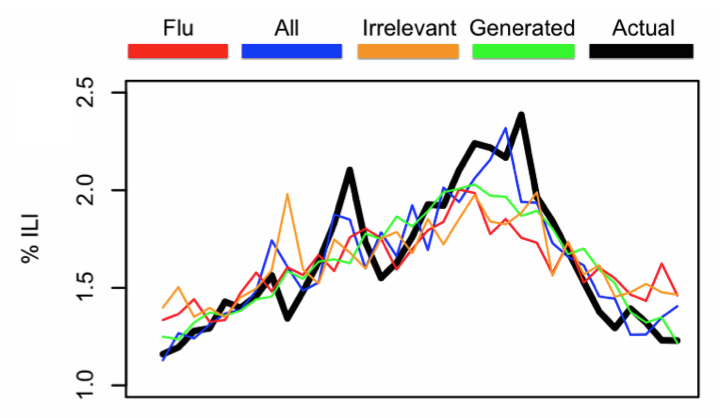
\includegraphics{introduction/figures/www2013_svmr.png}
\caption[SVM-regression for the 2011-2012 Influenza season using multiple datasets.]{SVM-regression for the 2011-2012 Influenza season using multiple datasets, from \cite{www2013}.}
\label{fig:intro_www2013}
\end{figure}


As mentioned above, GFT does not specifically differentiate between searches about \emph{having} influenza and \emph{news} about influenza. A similar issue occurs with Twitter analysis: rate limiting makes it impossible for a third party to gain \emph{all} tweets during a period of time. This is commonly addressed by searching for Tweets which contain keywords such as ``flu'' or symptoms of influenza. Note that this does not filter out Tweets about news about influenza, although work has been done in filtering out these messages \cite{culotta2010towards,lamb2013separating}. However, the bag-of-words approach for Twitter disease modeling has one major issue: we've been able to replicate the results from datasets based on flu keywords by using tweets that were collected using completely irrelevant search terms, specifically keywords related to zombies (see Figure \ref{fig:intro_www2013}).

Additionally, we've compared an unfiltered, random sample of tweets and generated time varying frequencies simply by 
\begin{equation}
x_{i,t} = (sin(t*\alpha_{i,1} + \alpha_{i,0})+\mathcal{N}(0,.1))/1000 + .001
\end{equation}
where \(\alpha_{i,0}\) and \(\alpha_{i,1}\) are randomly generated weights, \(\mathcal{N}(0,.1)\) is a normally distributed random variable with standard deviation of 0.1 and \(x_{i,t}\) is the value of curve \(i\) at time \(t\). While this is essentially building a model based simply off of the initial, disease frequency's time series, the fact that its performance is equivalent to more complex, data mining approaches brings the value of the later approaches into question. Further discussion and methods are available in chapter \ref{www2013}.

Besides human determined keywords, all papers surveyed do not encode any semantic knowledge into their models which may be one explanation for issues related to model generalization outside of the initial dataset.


\subsection{Obsession with Disease Tracking over Knowledge Generation}

Infectious disease studies using big data have strongly focused on surveillance systems \cite{world2006communicable} to either predict the future or current state of a disease's spread. \cite{gft,chunara2012new,culotta2010towards,goel2010predicting,signorini2011use,kim2013use} These models tend to strongly correlate with the actual disease's prevalence (for example, Yaari et al. \cite{yaari2013modelling} report \( r > .97\)) limiting the value of further optimizing these methods or the likelihood that improvements will be statistically significant. Other topics--such as disease transmission\cite{salathe2010high,Cauchemez:2011cp,Ferrari:2011ht}, the use of vaccines\cite{Salathe:2011gr,Wells:2013tp,Seale:2010br,Larson:2013kh,Bansal:2006di,Salathe:2008ct}, disease movement patterns\cite{Huang:2013ed,Balcan:2009ub,Afzal:2011bc}, behavioral effects of diseases\cite{Funk:2010cc,Jones:2009cv,Funk:2009ks} or the economic impact of diseases\cite{Tudor:2008kh,GruneYanoff:2011hl,Glasser:2004is}--are widely studied topics in traditional epidemiology, but have been neglected when it comes to big data analytics. This is particularly odd considering that the basis for these other topics, measurements of a population's illness, are also the basis for disease surveillance systems.

%While the WHO's definition of a surveillance system  includes ``response and control'' of a disease, it is unclear if providing real-time surveillance is much better than the CDC's current ILINet, which has a lag of 1 to 2 weeks. Instead, predictive models and work on designing influential messages about a disease may be more effective. Very little work has been put in to predicting future disease rates, possibly due to a much higher difficulty compared to models which  ``predict the present'' rate of disease. \cite{gft,chunara2012new,culotta2010towards,goel2010predicting,signorini2011use} Indeed, one of the few papers to attempt such a model ``demonstrated the inability of the prediction to follow the initial rise of the ILI data.''\cite{kim2013use} The issues regarding response and controll have been covered in part by advertising research, although more work on Tweets and messages specific to disease is needed \cite{timimi2013shape}.


\subsection{Inability to Influence Disease}

Using messages to influence behavior is a well studied technique,\cite{Eyssartier:2008jy,CavalliSforza:1982we,Rendell:2010go,Traulsen:2010ja,Centola:2010ki,Bond:2012ff} indeed it is the basis of the advertisement industry. However, work on public health messages has lagged more commercial topics \cite{timimi2013shape}. Work has generally focused on an individual's knowledge about a disease, as discerned through surveys\cite{Jones:2009cv} or a simple analysis of events\cite{Kinsman:2012wi}. While an understanding of the population's opinion on a topic can be the basis for crafting an influential message, it is a relatively primitive approach compared to large scale A/B testing \cite{bakshy2014www} or modeling a user's behavior using hundreds of thousands of variables. \cite{mcmahan2013ad}

\section{Proposed Solutions}
\subsection{On the ground validation through professional diagnoses}
\label{subsec:intro_uhs}
Others have worked on a top-down approach by using region-wide disease prevalence data from which Twitter data can be fit. \cite{gft,culotta2010towards,culotta2013lightweight,signorini2011use} However, they do not aim to say whether a specific Twitter user is ill, limiting the usefulness of such methods. In chapter \ref{www2014}, we consider a bottom-up approach to disease surveillance by diagnosing users based off of their Twitter information \cite{www2014}. To do this, we survey 104 people that were \emph{professionally} diagnosed with influenza through Penn State's University Health Services. As a control group, we survey an additional 122 individuals that were \emph{not} diagnosed with influenza. From this data, we were able to collect Twitter data from 104 users.

%To match other work, we started by considering Tweets that were filtered by keywords that a domain expert may choose: ``flu,'' ``influenza,'' ``sick,'' ``cough,'' ``cold,'' ``medicine'' and ``fever.'' While five of the keywords did provide some information, models based simply on these keywords did not perform well (see Figure \ref{fig:intro_www2014}, orange curve). Additionally, ``influenza'' appeared only once and was not in the context of the poster being ill. Thus, search terms that previous work \cite{culotta2010towards,signorini2011use} has considered useful does not seem to be very useful. 


%We also looked for user's that specifically said that they were sick with influenza-like symptoms. We hand rated all tweets during times when the users were sick, according to their medical records, and hand rated a subset of all other Tweets as a control. We found that half (\(17/35 \approx 48.6\%\)) of the users specifically mentioned their illness and we didn't find any users mentioning their influenza-like-illness in the control set. A significant signal, but we needed to find more for a true diagnostic system.

We employed machine learning algorithms such as naive Bayes and support vector machines to use the aggregated set of messages a user posted during the time that she was ill, or an equivalent aggregation when she was healthy, to attempt a diagnosis. Next we looked at non-message information. We performed anomaly detection on a user's rate of Tweeting to see if their usage changes when sick. We find a significant difference in activity, however the results are too noisy to be considered a viable method to diagnose influenza. We consider the aggregated messages from a user's friends \emph{followers} and perform text analysis on them, as was done on the user's messages. We find that a user's follows are a much stronger signal toward a user's health than the accounts that a user follows. This hints at the Twitter's network structure: I follow both celebrities and my friends, but only my friends follow me. Finally, we employ meta-classifiers which use the output of each of the previous classifiers discussed as an input for a final classifier to get better classifier accuracies.



%\begin{figure}
%\centering
%\begin{subfigure}{.3\textwidth}
%  \centering
% \includegraphics[width=.95\linewidth]{figures/measure/uhs_graph.png}
%\end{subfigure}
%\begin{subfigure}{.3\textwidth}
%  \centering
%  \includegraphics[width=.95\linewidth]{figures/measure/uhs_graph_with_others_with_singleton.png}
%\end{subfigure}
%\begin{subfigure}{.3\textwidth}
%  \centering
%  \includegraphics[width=.95\linewidth]{figures/measure/uhs_graph_with_others_no_singleton.png}
%\end{subfigure}
%\caption{The difference in scale between our network of users with professional diagnoses (left), and the network that is generated when their friends and followers are included (center) illustrates the value of employing less accurate data sources. By removing nodes with degree less than two (right) additional typology is visible.}
%\label{fig:measure_mininetwork_full}
%\end{figure}

\section{Quantifying Disease Dynamics}
In chapter \ref{longitude}, we combine this classifier with a dataset of 2.7 billion Tweets to track 16 million users' disease states over a period of four years. Additionally, we employ geographical analysis of the users' supplied location information to approximate his real-world social network, \cite{hawelka2014geo,leetaru2013mapping,tatem2014mapping} specifically with respect to disease, which has previously been approached through measuring real world contacts. \cite{isella2011close,salathe2010high,smieszek2014should} We do this by seeing if other users near a given user can inform us about the given user's future health status. That is, are they likely to get sick when people near them have recently been sick?

This question can be answered based on probabilities, but instead we decide to model it based on the base reproduction rate, \(R_0\). This rate is the basis of most disease spread models, however, it is generally calculated by fitting curves to measured disease prevalence rates.\cite{yang2015inference} Attempts to study peer to peer transmission are limited in size (generally by the costs of tracking a group's disease states) to either 10's or 100's of individuals\cite{Cauchemez:2011cp,moser1979outbreak,klontz1989outbreak,salathe2010high}. Instead, we exploit an already developed social network platform, Twitter, as the basis of our collection, allowing us to preform these studies at web-scale.

%We consider using this data and classifier to add to work about whether or not a user's network on Twitter can be used to approximate his real-world social network, \cite{hawelka2014geo,leetaru2013mapping,tatem2014mapping} specifically with respect to disease, which has previously been approached through measuring real world contacts. \cite{isella2011close,salathe2010high,smieszek2014should} We do this by seeing if a user's friends' and followers' health statuses can inform us about the user's own health. That is, are they likely to get sick when their friends on Twitter are sick? Optimally, we would just use the accounts on which we have a professional diagnosis, but it appears that there is not enough data. Only 30 accounts share direct links between each other. Thus, we will also use the 913,082 accounts that either follow or are followed by our gold-standard users (for a visual representation of the difference in scale, see Figure \ref{fig:measure_mininetwork_full}). These users can be diagnosed by applying the methods described above.

\section{Targeting Messages towards Disease Related Individuals}

In chapter \ref{retweets}, we consider the effects of various aspects of a message on retweeting rates, a signal for reader interest.\cite{Suh:2010uw,Kim2012retweet,Stieglitz2012politics,gransee2012} We consider network structure, the type of user that posted a message and the textual content of the message. Additionally, sentiment analysis is often used to measure how positive or negative a message is.\cite{Kim2012retweet,Stieglitz2012politics,Zhao:2012vz,Bollen:2011wv,Ofek:ug} Again, this has been shown to be a signal for retweeting rates. However, in the case of disease information, messages tend to be predominately negative. Instead, we develop a model based on four dimensions of emotional content\cite{russell1977evidence,plutchik2001nature,Cambria2011} and apply it towards the retweet prediction problem.
\include{twitterFitting/paper}


\chapter[On the Ground Validation of Online Diagnosis with Twitter and Medical Records]{On the Ground Validation of Online Diagnosis with Twitter and Medical Records\footnote{A version of this chapter \cite{Bodnar:2014:GVO:2567948.2579272} was previously presented at WWW2014, \textcopyright 2014 International World Wide Web Conferences Steering Committee. }}
\label{www2014}

%The right, after publication by IW3C2 and ACM, to use all or part of the Article and abstract, without revision or modification, in personal compilations or other publications of the author's own works, and to make copies of all or part of such materials for the author's use for lecture or classroom purposes (excluding the preparation of course pack material for onward sale by libraries and institutions), provided that the first page of such use or copy prominently displays the bibliographic data and the following copyright notice: '© [year] International World Wide Web Conferences Steering Committee’
%see http://www2009.org/files/IW3C2.pdf

%\begin{abstract}
%Social media has been considered as a data source for tracking disease.  However, most analyses are based on models that prioritize strong correlation with population-level disease rates over determining whether or not specific individual users are actually sick. Taking a different approach, we develop a novel system for social-media based disease detection at the individual level using a sample of professionally diagnosed individuals. Specifically, we develop a system for making an accurate influenza diagnosis based on an individual's publicly available Twitter data. We find that about half (\(17/35 = 48.57\%\)) of the users in our sample that were sick explicitly discuss their disease on Twitter. By developing a meta classifier that combines text analysis, anomaly detection, and social network analysis, we are able to diagnose an individual with greater than 99\% accuracy even if she does not discuss her health.
%\end{abstract}
%\footnotetext{hello}Bodnar:2014:GVO:2567948.2579272
\section{Introduction}
%Digital epidemiology, datamining Internet records to approach epidemological questions in novel ways, has recently been proposed as an alternative to traditional disease surveillance methods[]. 

Disease surveillance systems -- which traditionally rely on reports from medical practitioners -- are an important part of disease control. However, these traditional surveillance systems are often costly and slow to respond \cite{Chan2010,Heymann:2001,Salathe:2012ez}.  The widespread adoption of the Internet by the general public has provided opportunities for the development of novel disease surveillance methods. Compared to traditional systems, where data is provided by medical diagnosis, these new systems provide either semi-automatic -- through long term self reporting systems \cite{Marquet:2005tb,VanNoort:2007uk} -- or fully automatic -- through data mining search queries or social media \cite{Bodnar:2013we,Butler:2013uh,Culotta:2010hx,Goel:2010jf,Olson:2013bo} -- disease surveillance. While these methods are cheaper, faster and cover a larger number of individuals than traditional systems, one can be less confident about their results than the results from a system based on professional diagnosis. In this paper, we develop a system that performs long term surveillance on Twitter users with classifiers trained on professionally diagnosed data that combines the advantages of all three of these systems.

Previous work with data mining social media has focused on methods to replicate the patterns found in traditional surveillance networks \cite{Bodnar:2013we,Culotta:2010hx,Goel:2010jf}. However, these methods have several limitations. First, they generally do not differentiate between an individual with an illness and an individual that is worried about an illness; which may have resulted in a predicted influenza rate that was much higher then the actual 2013 influenza rate \cite{Bodnar:2013we,Butler:2013uh,Lamb:2013to,Olson:2013bo}. Second, these methods cannot be extended to areas without a previous surveillance network to train the model. Finally, these methods are fundamentally incapable of detecting diseases that do not show strong spatial-temporal patterns such as mental illness, obesity or Parkinson's disease. Instead of top-down methods to measure levels of disease in a population, we approach this problem from the bottom-up. This addresses all three of these issues: we only diagnose individuals that are likely to have the disease, and not just interested in the disease; we do not require previous data when applying these methods to new problems or locations; and these methods can easily generalize to diseases that do not show strong spatial or temporal patterns because we focus on an individual level.

Participatory systems, such as InfluenzaNet or Flu Near You, use self-reported symptoms to diagnose an individual and also work from a bottom-up approach \cite{Marquet:2005tb,VanNoort:2007uk}. These systems have the potential to be better than traditional surveillance systems because they update in near-real-time and can detect cases even when the user has not gone to their doctor. These systems require the user to sign up which allows for long term studies which are not normally able to be done with Tweets or search queries. However this reduces the number of users studied compared to data mining approaches. For example, Flu Near You had a total of 9,456 users report during the week ending on 29 December 2013. Marquet et al. \cite{Marquet:2005tb} have shown a large drop out rate with only 53\% of users participating for five or more weeks. While this amount of data is sufficient for many purposes, a system based on Twitter's millions of active users would open the door to more applications.


%Digital epidemiology \(\to\) novel disease detection mechanisms.
%
%Validation of this idea is important, but not done.
%
%Pull med info of individuals professionally diagnosed with ILI and their twitter accts. Compare old methods. Suggest some new things.

We develop such a system as follows. In section 2 we describe the collection of an individual's professional diagnoses of influenza and the collection of their Twitter information. In section 3 we consider extracting textual information from Tweets as a method for diagnosing influenza. Previous work has focused on this area. Additionally, we consider other methods for detection. In section 4 we consider anomalies in a user's Tweeting behavior as a signal for diagnosing influenza. In section 5 we extend these methods to other users on a person's social network to diagnose the original person. In section 6 we aggregate the results of the previous classifiers to develop a more accurate meta-classifier.

%\section{Related Work}

%People with issues \cite{Bodnar:2013we,Butler:2013uh,Lamb:2013to} also plos paper!

%Most work to this point considers finding messages in tweets (i.e. ``I'm sick'') or in keyword frequencies. 

%Tweet classification \cite{Culotta:2010hx,Lamb:2013to,Salathe:2011gr}
\begin{figure} [h]
\centering
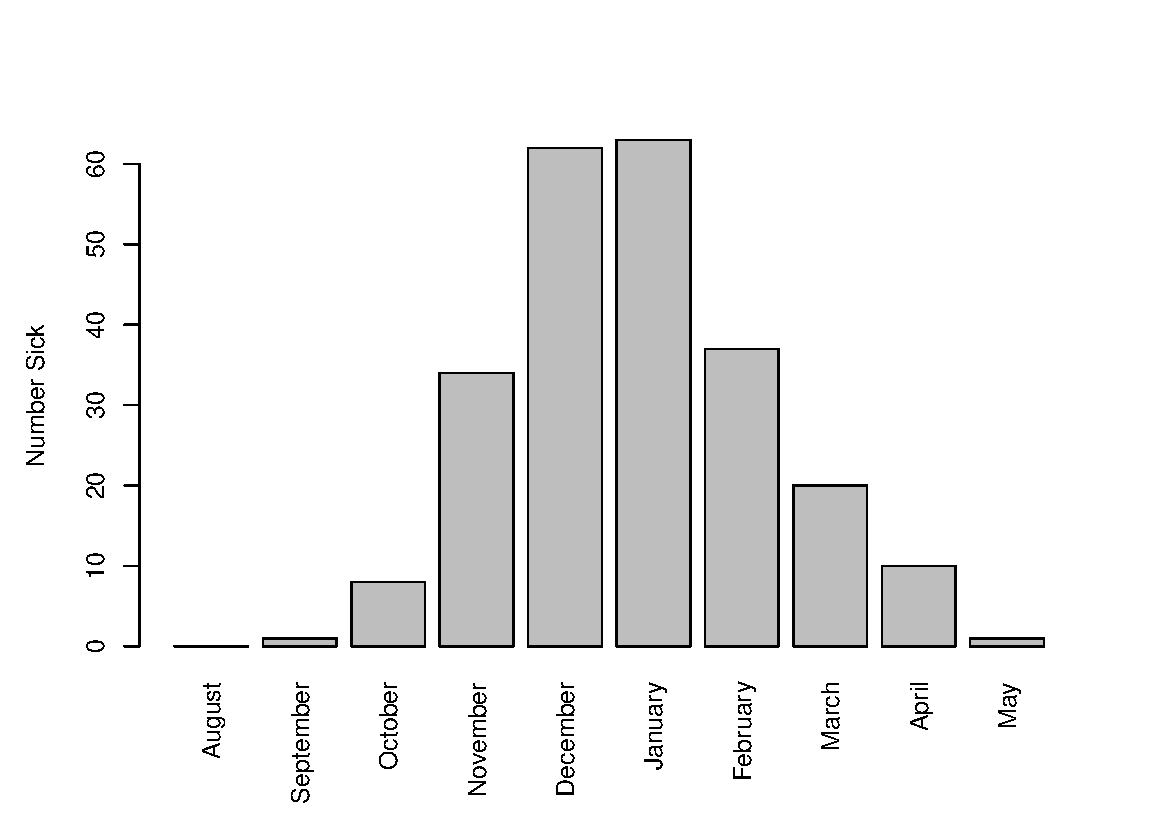
\includegraphics[width=.9\textwidth]{diagnosis/figs/sick_count.eps}
\caption{The professionally diagnosed Influenza cases during the 2012-2013 season in our sample.}
\label{fig:flu_rate}
\end{figure}
\section{Data Collection}
\subsection{Medical Records}
We received information from the Pennsylvania State University's Health Services about 104 individuals that were diagnosed with influenza by a medical professional during the 2012-2013 Influenza season. Due to privacy concerns, we were limited to knowing which month an individual was diagnosed (see figure \ref{fig:flu_rate}).  For comparison, we also obtained information from 122 individuals that were \emph{not} diagnosed with influenza during this time. The participants were mostly students (\(72\%\) were between the ages of 18 and 22) and slightly more female than expected (\(133 / 226 \approx 58.8\%\).) Data collection was approved through the Pennsylvania State University's IRB (approval \#41345.) Twitter handles were available for 119 of these individuals.

\subsection{Twitter Records}
While we received a total of 119 Twitter accounts, 15 were discarded because the associated accounts were either non-existent, banned or private. For each of the remaining 104 accounts, we pulled their profile information, their friends and followers information, their most recent 3000 tweets, and their friends' and followers' profiles and tweets. Some users did not tweet during the month that they were sick; we kept those accounts as part of the control group. We were limited to the most recent 3000 tweets by Twitter's time line query, but this only effected two accounts -- both of which posted multiple times per hour and were thrown out because we could only look back a few days.

We collected data through the Twitter API. Tweets, profile and follower information queries have separate rate limits and were collected in parallel. Since users continued to Tweet during data collection, each account was queried no more than once every three days for new Tweets. When all accounts could not be queried due to rate limiting, the accounts that had been queried the least recently were updated. Additionally, the 104 seed accounts collected above were given higher priority over their friends and followers. In total, we collected 37,599 tweets from the seed accounts and 30,950,958 tweets from 913,082 accounts that they either followed or were followed by.

%select count(distinct(d_net.user)) from (select distinct(user) as user from tweets_network) as d_net left join tweets on d_net.user = tweets.user where tweets.user is null;

%\section{Signal Detection}
\section{Text Based Signals}
\label{sec:text_analysis}

In this section, we consider diagnosis based on the content of a user's tweets. Such analysis can be approached by keyword analysis, where the presence of absence of a keyword predicts disease, or through text classification, where the tweets are classified as being about disease or not about disease. We begin by dividing the tweets into two sets: tweets that were posted the same month that a user was sick and tweets that were posted other times. We find a total of 1609 tweets from 35 users in the first category.

\begin{table}[h]
\centering
\begin{tabular}{|c|c|c|c|} \hline
Word& Total &Odds Ratio & Significance\ \\ \hline
flu&25&40.14& \textless 0.0001 \ \\ \hline 
influenza&1&0.00&0.8325\ \\ \hline 
sick&128&5.22& \textless 0.0001 \ \\ \hline 
cough&18&4.48&0.0094\ \\ \hline 
cold&82&1.45&0.4154\ \\ \hline 
medicin&9&11.20& \textless 0.0001 \ \\ \hline 
fever&13&26.20& \textless 0.0001 \ \\ \hline 

\end{tabular}
\caption{Probability of keywords being Tweeted by a user during the month that he or she was diagnosed with influenza.}
\label{tab:tweet_keyword_expert_results}
\end{table}

First, we use the occurrence or absence of keywords as features for classification. A set of keywords are defined that are possibly signals of influenza. We chose \{flu, influenza, sick, cough, cold, medicine, fever\} as our set of keywords. These keywords include the names and symptoms of the illness in addition to ``medicine'' and serve as a set of keywords that may have been chosen by a domain expert. We use Fisher's exact test to compare keyword occurrence in months when the user is sick or not sick and find a significant effect for six of the seven keywords (See table \ref{tab:tweet_keyword_expert_results}). Additionally, we try algorithmically selecting keywords by first finding the 12,393 most common keywords in the data set (words that occur atleast twice).  We then rank them based off of information gain on predicting influenza and choose the top 10, 100 or 1000 keywords from the list. A list of the most statistically significant, positive signals is available in appendix \ref{appendix:keyword_recommendations}. In all of these cases, we pre-process the data by tokenizing the text on spaces, tabs and line breaks and the characters ``.,;':"()?!/\textbackslash '', remove stop words\footnote{Stop words were taken from Weka's stop list version 3.7.10.}, perform Porter stemming \cite{Porter:1980dd}  and convert the text to lower case. We use Naive Bayes, random forest, J48 (a Java implementation of C4.5), logistic regression and support vector machines to classify a user as being sick in a given month or not (see figure \ref{fig:roc_keyword}).



\begin{figure} [h]
\centering
\begin{subfigure}[b]{.4\textwidth}
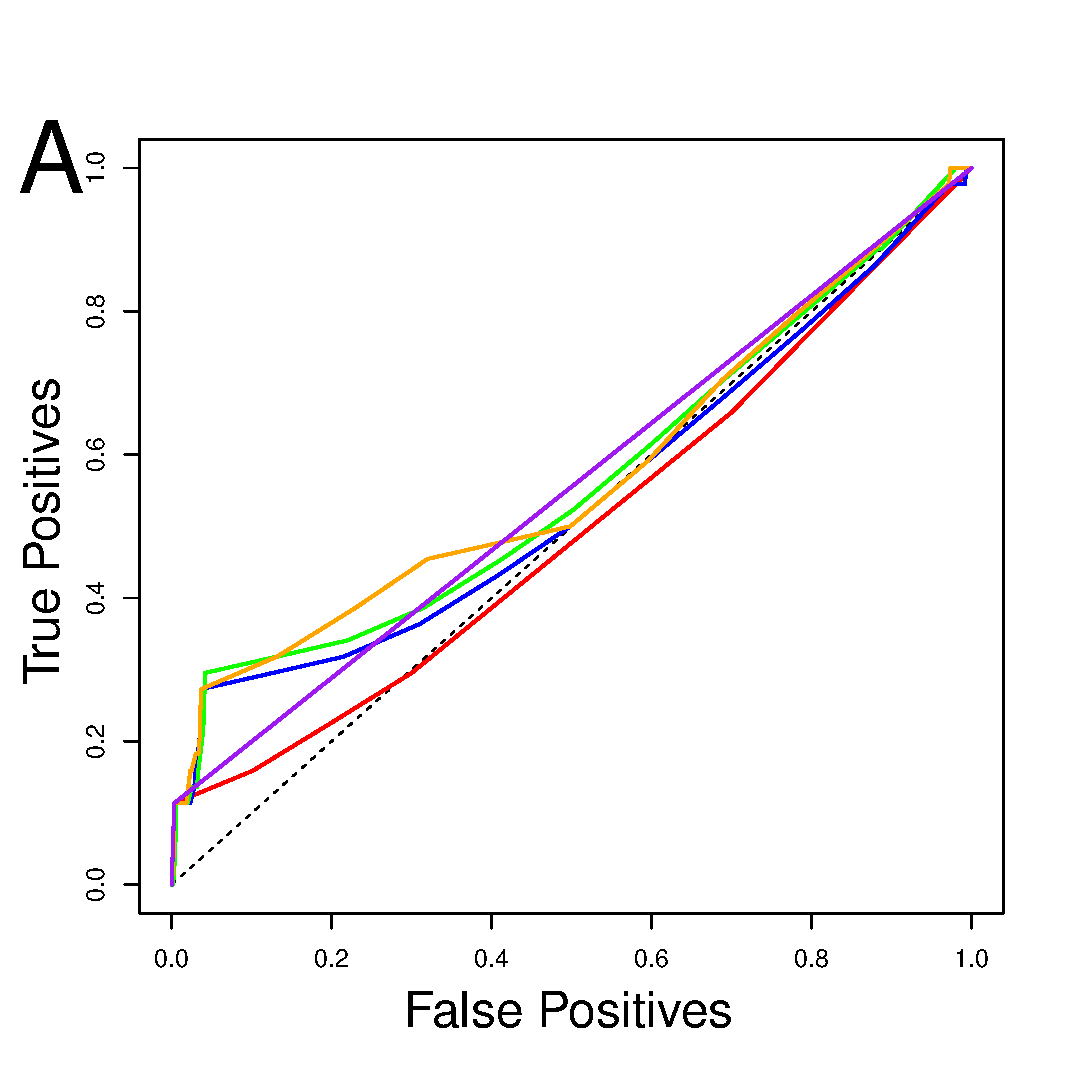
\includegraphics[width=\textwidth]{diagnosis/figs/key_exp_roc.eps}
\end{subfigure}
\begin{subfigure}[b]{.4\textwidth}
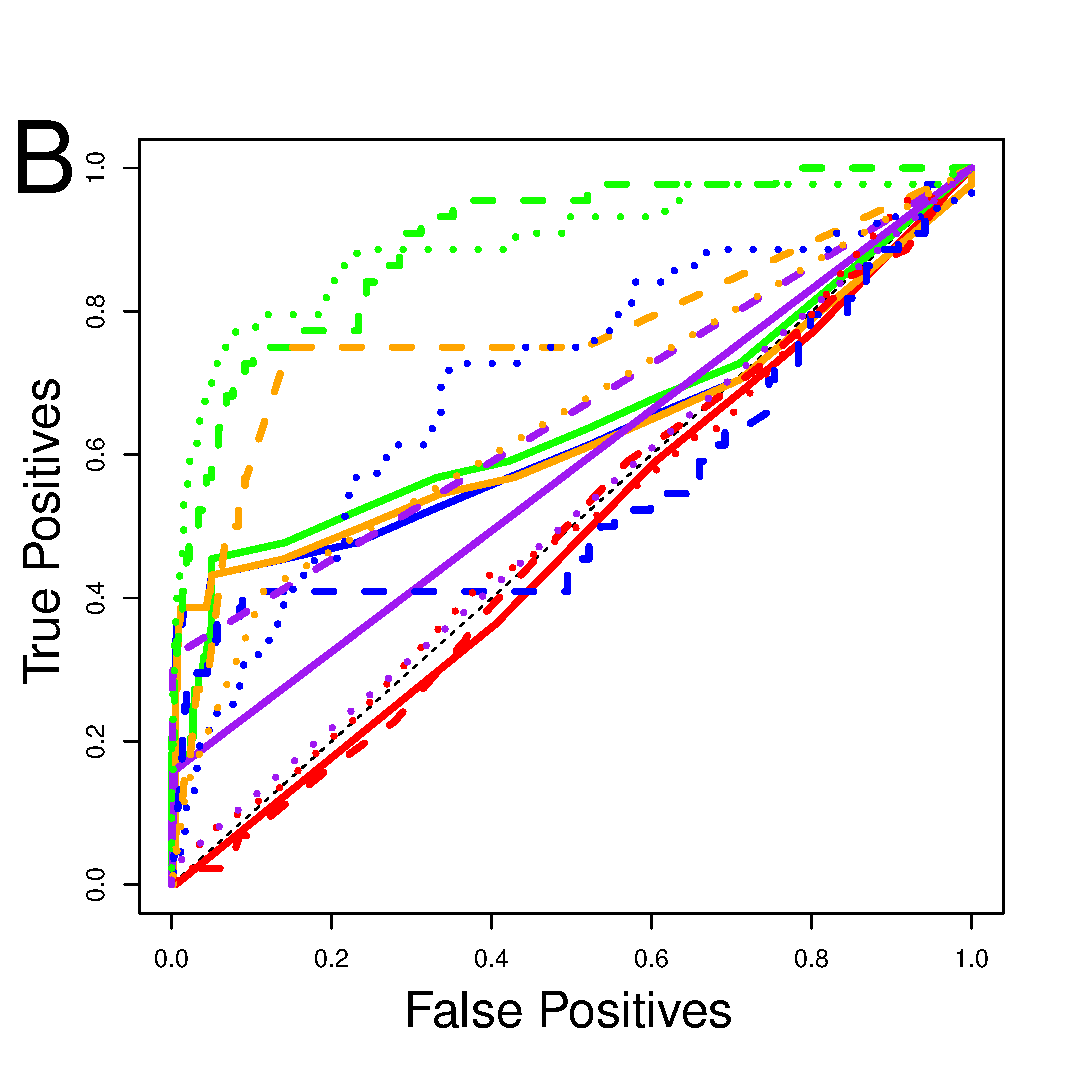
\includegraphics[width=\textwidth]{diagnosis/figs/key_dm_roc.eps}
\end{subfigure}
\begin{subfigure}[b]{.9\textwidth}
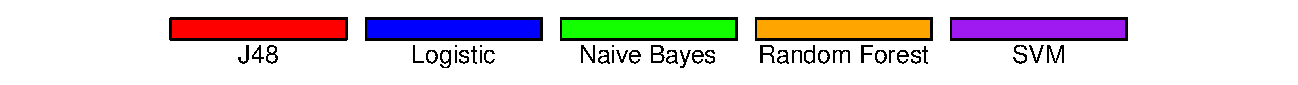
\includegraphics[width=\textwidth]{diagnosis/figs/keyword_legend.eps}
\end{subfigure}
\caption{The ROC of classifiers that use hand chosen keywords (a) and algorithmically chosen keywords (b) to determine if an individual is ill. The top 10 (solid line), 100 (dashed line) and 1000 (dotted line) were selected as the features.}
\label{fig:roc_keyword}
\end{figure}


Second, we consider analysing the content of a tweet's text for messages giving hints about being sick such as ``another doctor's appointment Wednesday ... have to \#treatmyflu'' or ``I didn't realize how bad it feels to have the flu, should have gotten a flu shot\footnote{These examples are based off of real tweets, but changed to keep our participants anonymous.}'' that would not be detected through simple bag-of-words techniques. Computational approaches for natural language processing are available. However, because our dataset is relatively small, we use a `human' classifier by hand rating all 1609 tweets that were posted by individuals during the time of their illness. We also sample a randomly selected set of 1609 tweets from times when the users did not have influenza as a control. We find 58 tweets from 17 (\(17/35 = 48.57\%\))  individuals in our study that are about the user being sick. We also find zero tweets about the user having influenza during times when they did \emph{not} have influenza. Because humans are very good at extracting information from text, hand rating tweets allows for an approximately 100.0\% accurate classification, although it clearly does not scale well. Extracting information from text using machine learning is a complex problem where finding solutions that perform as well as humans is rare. Thus, the human classifier gives us an upper limit to the accuracy of a health monitoring system based off of tweet classification (see table \ref{tab:tweet_classified_confusion}.)

\begin{table}
\centering
\begin{tabular}{|c|c|c|} \hline
Sick&Not Sick&\ \\ \hline
17 & 18 & Sick\\ \hline
0 & 66  & Not Sick\\
\hline\end{tabular}
\caption{Confusion matrix of a Tweet-Classification based diagnosis system. Rows are of true values, columns are of predicted values.}
\label{tab:tweet_classified_confusion}
\end{table}

\section{Frequency Based Signals}

In addition to illness affecting the content of individuals' tweets, it is likely that illness also affects the rate at which individuals tweet. To detect this, we perform one-dimensional anomaly detection on each user's monthly tweeting rate as follows. First, we calculate the number of tweets in each month in the study period and discard any months where the user tweets less than ten times. This avoids issues caused by the user starting or stopping their use of Twitter. We then calculate the z-score of the tweeting rate of the month that the user is ill by
\begin{equation}
z = \frac{|x - \bar{x}|}{\hat{s}}
\end{equation}

Where \(\bar{x}\) and \(\hat{s}\) are the estimated mean and standard deviation of the user's tweeting rate for each month during the study \cite{Grubs:1969ab}. We repeat this process for months when the user is not sick. We then classify the user as sick if \(z > 1.411\) where \(1.411\) was chosen through leave one out cross validation. We find a significant difference between the z-scores for months when a user had influenza and months when the user did not (\(p = 0.01303\), two-sample Kolmogorov-Smirnov test). Most of the time individuals are not sick (219 / 258 = 84.88\% of the months), resulting in a highly biased sample. Thus we optimize based on the \(F_1\) score instead of accuracy. The optimal z-score cutoff results in  an area under the ROC curve of .6218 and \(F_1= 35.0\%\). (See table \ref{tab:tweet_anomaly_confusion}.) 

%\begin{figure} %need to redo
%\centering
%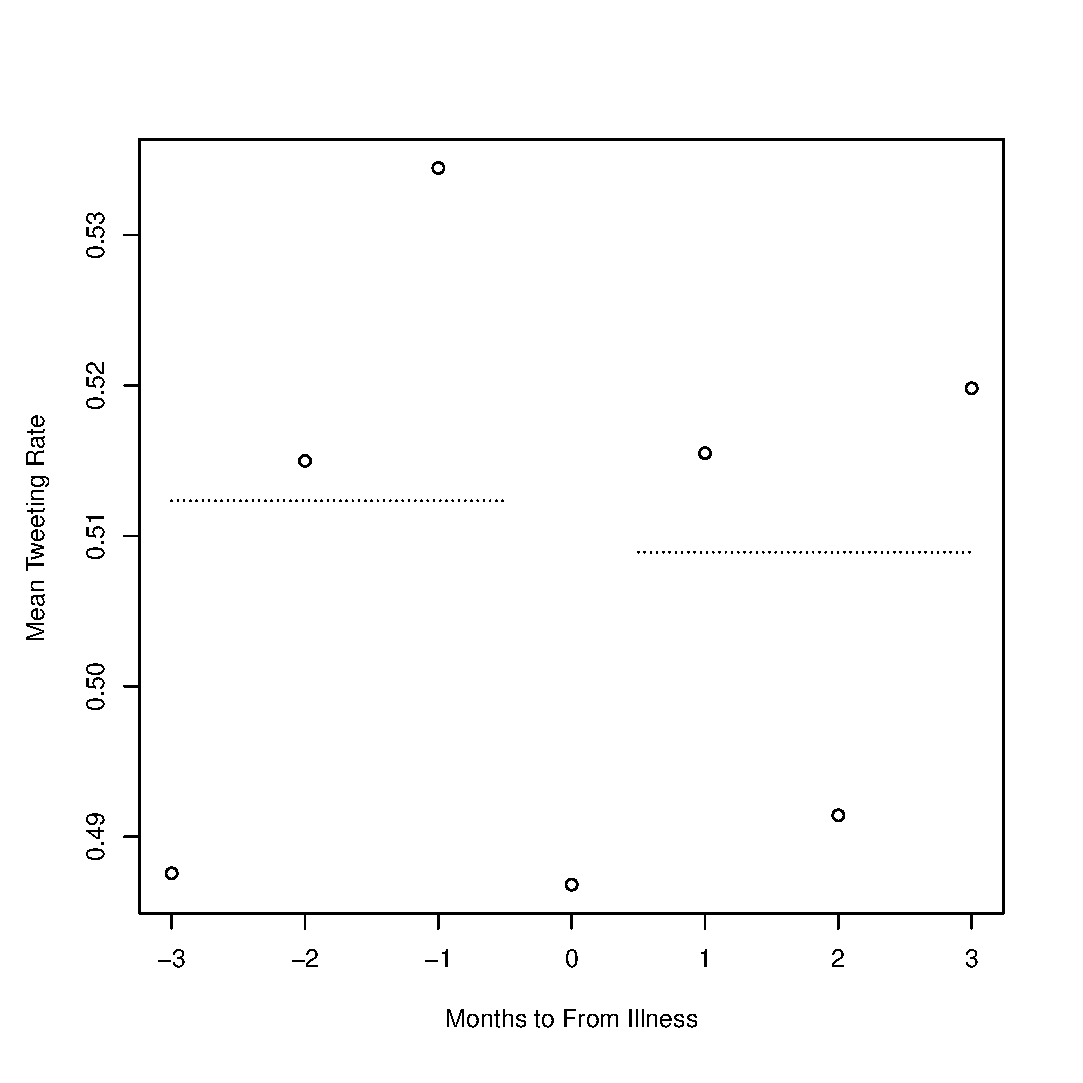
\includegraphics[width=0.5\textwidth]{figs/meanFrequencies.eps}
%\caption{The frequency of tweeting behaviour of individuals in the months before, during and after an illness. Users significantly (check) decrease their rate of tweeting during the time that they had influenza. Dashed lines indicate the mean rate for the three months before / after the illness. (Todo: check significance)}
%\label{fig:mean_freq}
%\end{figure}

\begin{table}[h]
\centering
\begin{tabular}{|c|c|c|} \hline
Sick&Not Sick&\ \\ \hline
14 & 25 & Sick\\ \hline
27 & 192 & Not Sick\\
\hline\end{tabular}
\caption{Confusion matrix of the classifier based on anomalous tweeting rates. Rows are of true values, columns are of predicted values.}
\label{tab:tweet_anomaly_confusion}
\end{table}

\section{Network Based Signals}

Even if a user is not currently active on Twitter, users on her social network may give clues to her health status. Twitter's social network is one directional, allowing for users to follow other users without the other users having to follow them back. Accounts that follow a user are referred to as her `followers,' and accounts that a user follow are referred to as her `friends.' We consider all text that a user's friends or followers tweeted and perform keyword analysis. The analysis was performed the same way as we analyzed the user's tweets in section \ref{sec:text_analysis}, except we normalize the counts here by the total number of characters her followers or friends tweeted. This controls for the number and activity of a users friends or followers, which should not have an effect on her health status. We find that most of the tested classifiers are able to detect a signal in both the user's followers' and friends' streams (see figure \ref{fig:roc_network}.)


%follower 12393
%friend 11595
%best = nb_1000 roc=.8641
\begin{figure} [h]
\centering
\begin{subfigure}[b]{.4\textwidth}
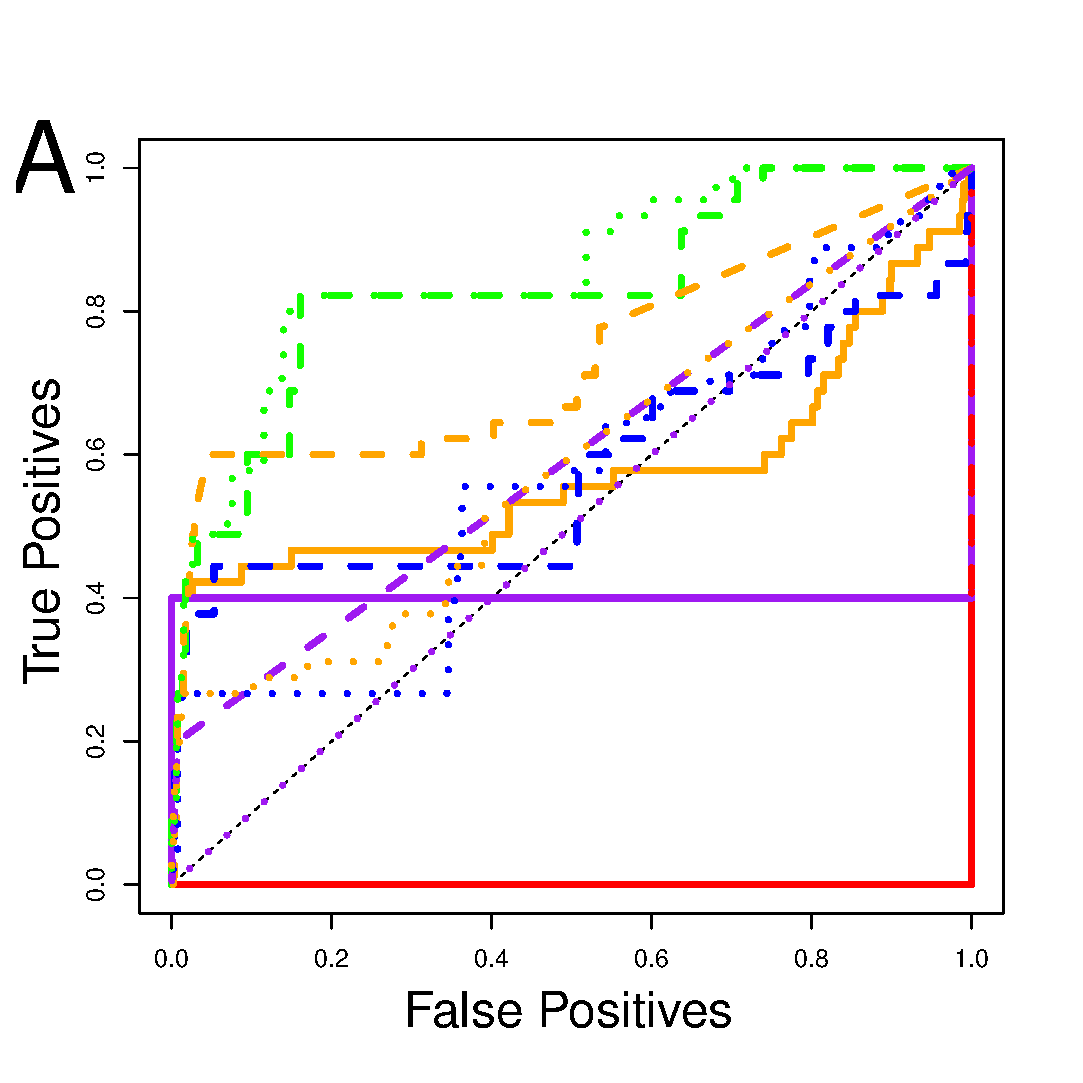
\includegraphics[width=\textwidth]{diagnosis/figs/followers_roc.eps}
\end{subfigure}
\begin{subfigure}[b]{.4\textwidth}
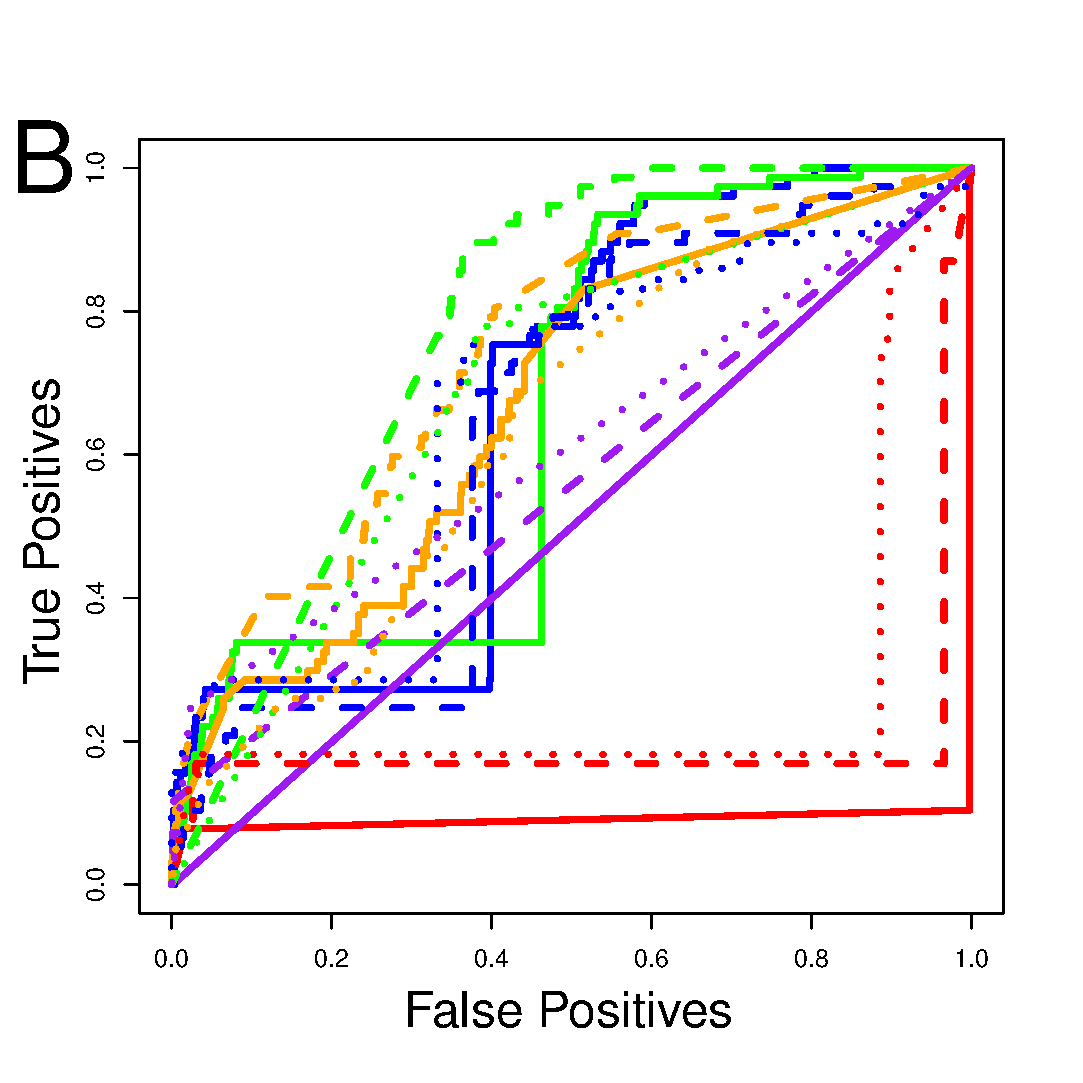
\includegraphics[width=\textwidth]{diagnosis/figs/friends_roc.eps}
\end{subfigure}
\begin{subfigure}[b]{.9\textwidth}
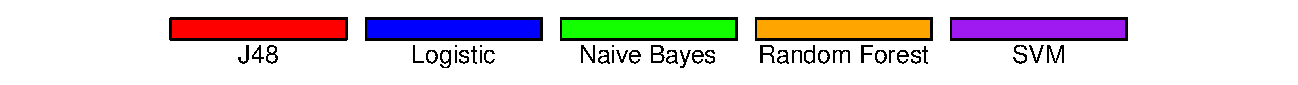
\includegraphics[width=\textwidth]{diagnosis/figs/keyword_legend.eps}
\end{subfigure}
\caption{The ROC of classifiers based off Tweets from (a) accounts that follow a user and (b) accounts that a user follows. Line coloring and style are equivalent to figure \ref{fig:roc_keyword}.}
\label{fig:roc_network}
\end{figure}

We further analyse the strength of these classifiers by building each classifier using 10 fold cross validation and calculate their performance by measuring area under the ROC curve. We repeat this 100 times to generate a distribution of each classifier's performance. We then perform an analysis of variance test to examine the differences between the sources of data (followers or friends), the number of keywords used and the classifier's algorithm (see table \ref{tab:network_aov}.) We find that the choice in classifier and the length of the feature vector have a significant effect on performance. We find that classifiers that use tweets from accounts that follow the user are significantly better at diagnosing the user than classifiers that use tweets from accounts that the user follows. This may be because Twitter users often follow celebrities and news organizations -- and celebrities and news organizations rarely follow personal Twitter accounts --  which could introduce excess noise. 

\begin{table}[htp]
\begin{center}
\begin{tabular}{llllll}
\hline\hline
\multicolumn{1}{c}{ }&\multicolumn{1}{c}{Df}&\multicolumn{1}{c}{Sum Sq}&\multicolumn{1}{c}{F value}&\multicolumn{1}{c}{Pr(\textgreater F)}\tabularnewline
\hline
Source&1&107.16&1290.82&\textless \(2^{-16}\) \tabularnewline
Keyword Size&1&72.19&869.66&\textless \(2^{-16}\)\tabularnewline
Classifier&3&752.55&3021.61&\textless \(2^{-16}\)\tabularnewline
Residuals&109194&9602& & \tabularnewline
\hline
\end{tabular}
\end{center}
\caption{Results from an analysis of variance of the area under the ROC curve for classifiers based on tweets from an individual's social network. Factors are whether the data is from the user's friends or followers, the number of keywords chosen and the classifier. }
\label{tab:network_aov}
\end{table}
\section{Meta Classifier}

So far we have considered five separate methods for detecting illness based off of a user's Twitter activity: hand-chosen keyword analysis, datamined keyword analysis, hand classified tweets, anomaly detection and network analysis. However, there is no reason that we cannot combine these methods to get a stronger signal. For example, while mining the user's text is the best of the five methods, she may stop tweeting while sick, which would be detected by the frequency-based anomaly classifier. Aggregating multiple classifiers by a `meta-classifier' has been shown to be an effective method for increasing classification accuracy \cite{Todorovski:2003hk,Frossyniotis:2004wx}.

\begin{table}
\centering
\begin{tabular}{|c|c|c|} \hline
Classifier&Area under ROC& Accuracy \\ \hline
AdaBoost & .9961 & 99.53\\ \hline
Bayesian & .9078 &  92.08\\ \hline
Decision Tree & .9877 & 99.22\\ \hline
Logit Boost & .9986 & 99.22\\ \hline
Weighted Voting & .9783 & 93.17\\ \hline
Baseline & .8544 & 89.72\\ 
\hline\end{tabular}
\caption{Performance of the meta classifiers. The presented baseline is the classifier based on datamined keywords -- the highest preforming individual classifier.}
\label{tab:meta_results}
\end{table}

We start by selecting the classifier from each of the previous five approaches that has the largest area under the ROC curve (see figure \ref{fig:roc_meta}.a.) We then use the predicted distributions from these classifiers as the feature vector for the meta classifier. We use Ada Boost, Bayesian classification, J48 decision trees, logit boost, and weighted voting to evaluate the meta-dataset. We then evaluate these methods with leave-one-out cross validation and see an increase in area under ROC and accuracy compared to the best individual classifier (see figure \ref{fig:roc_meta}.b.) We find that AdaBoost has the highest accuracy (99.53\%) and logit boost has the highest area under it's ROC curve with .9986 (see table \ref{tab:meta_results}.)

%adaboost, weighted voting, logistic, j48 decision trees, basian model, stacking, logit boost

\begin{figure} [h]
\centering
\begin{subfigure}[b]{.4\textwidth}
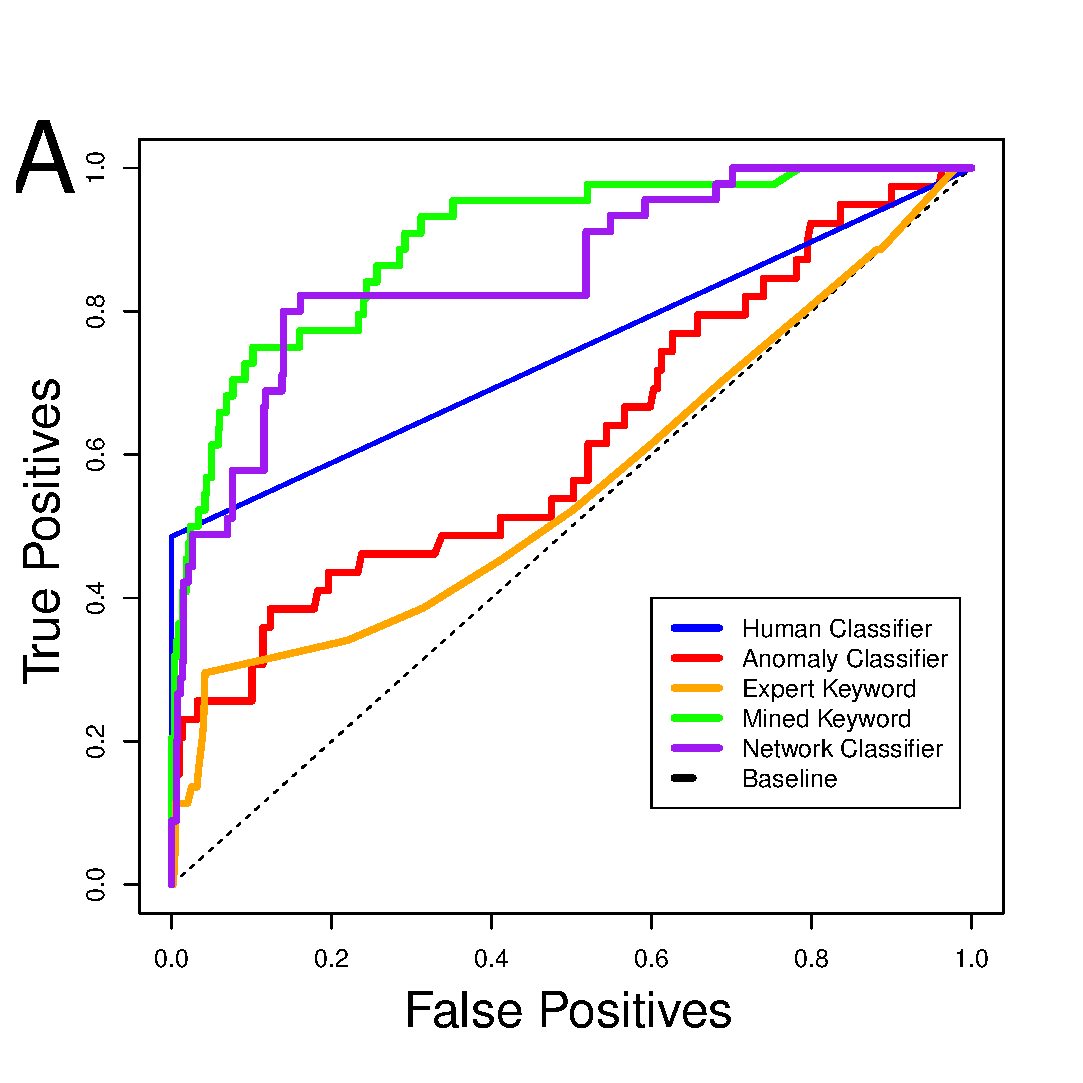
\includegraphics[width=\textwidth]{diagnosis/figs/meta_roc.eps}
\end{subfigure}
\begin{subfigure}[b]{.4\textwidth}
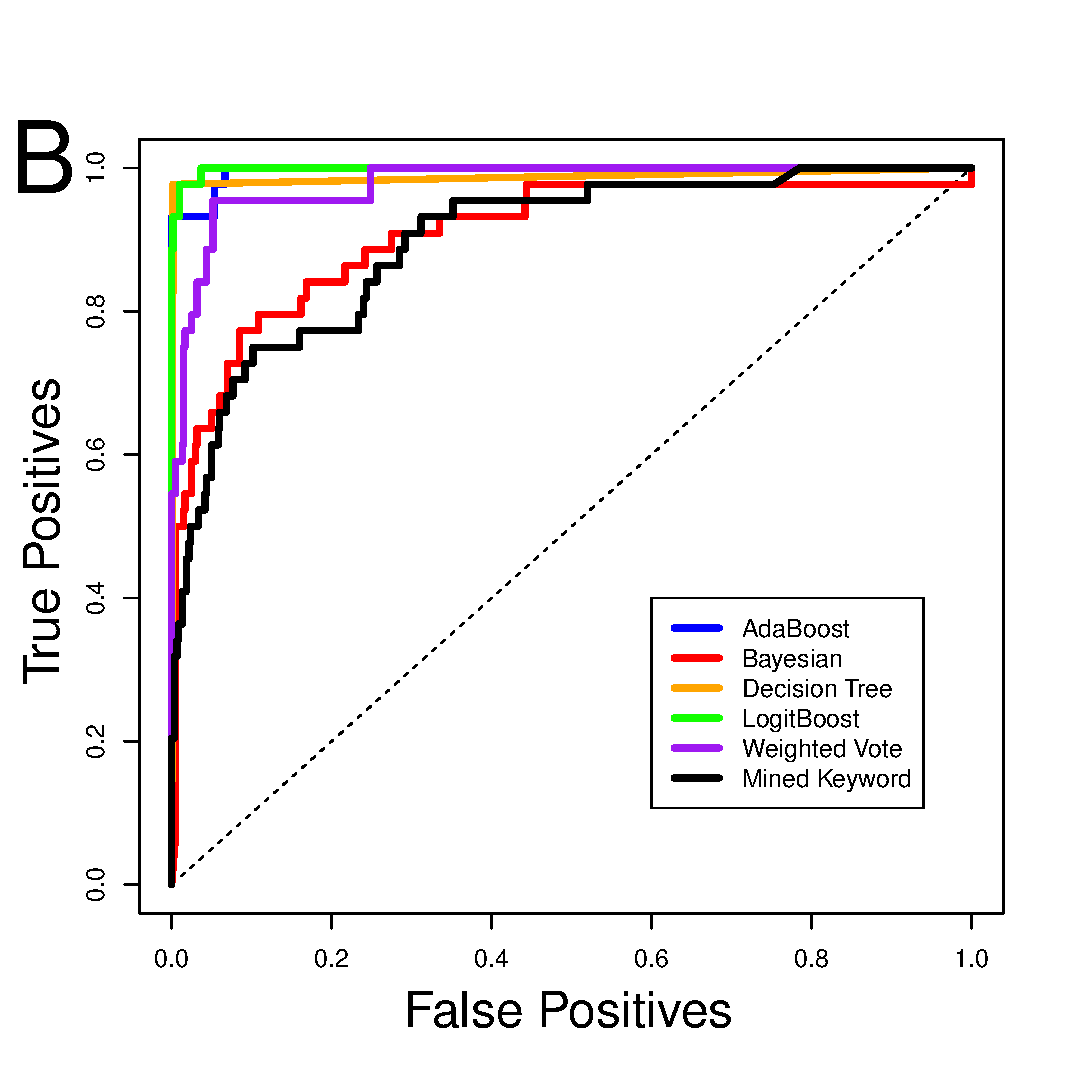
\includegraphics[width=\textwidth]{diagnosis/figs/meta_roc_final.eps}
\end{subfigure}
\caption{The accuracy of the previous classifiers (a) and the accuracy of various classifiers that use the previous classifier's results as features (b). }
\label{fig:roc_meta}
\end{figure}

\section{Conclusions}


In this paper, we have shown that it is possible to diagnose an individual from her social media data with high accuracy. Computational approaches to aid in disease diagnosis has been approached before, however they have been developed with a medical setting in mind. That is, the question addressed was ``can we diagnose an individual based off data gathered from medical tests run on her?'' instead of ``can we diagnose an individual solely based off of publicly available social media data?''  While we focus on the relatively benign case of remotely reconstructing a confidential diagnosis of influenza, these methods could also be applied to stigmatized diseases, such as HIV \cite{cosme2015}, where being able to determine if an individual is HIV positive without her knowledge and with only her Twitter handle could result in serious social or economic effects. Half of the users explicitly stated that they were sick, and we were able to confidently determine illness in the other half of the cases through their data. It would seem that simply avoiding discussing an illness is not enough to hide one's health in the age of big data. 

%\section{Conclusions}
%\begin{table}[!ht]
%\centering
%\begin{tabular}{|c|c|}\hline
%Keyword&Ratio\ \\ \hline
%flu &  34.424\\ \hline
%health &  11.360\\ \hline
%sick &  5.019\\ \hline
%track & 10.952 \\ \hline
%stud & 3.508 \\ \hline
%asshol & 9.090 \\ \hline
%ton & 9.090 \\ \hline
%particip & 20.667 \\ \hline
%salt & 20.667 \\ \hline
%recov & 40.118 \\ \hline
%fuck & 2.963 \\ \hline
%sham & 13.64 \\ \hline
%row & 10.180 \\ \hline
%win & 2.947 \\ \hline
%rt & 3.077 \\ \hline
%  \end{tabular}
%  \hspace{1em}
%\begin{tabular}{|c|c|}\hline
%cont. & \\ \hline
%walk & 3.077 \\ \hline
%childr & 6.820 \\ \hline
%incred & 6.820 \\ \hline
%meal & 6.820 \\ \hline
%longer &  6.820 \\ \hline
%succes &  26.765 \\ \hline
%accis & 26.765 \\ \hline
%holida & 26.765 \\ \hline
%luv & 26.765 \\ \hline
%oblig & 26.765 \\ \hline
%path & 26.764 \\ \hline
%pract & 26.764 \\ \hline
%prayer & 26.765 \\ \hline
%reserv & 26.765 \\ \hline
%riot & 26.765 \\ 
%\hline\end{tabular}
%\caption{The thirty keyword stems with the highest positive predictive power ranked by significance. The Twitter API limits searches to at most thirty keywords. Ratio is calculated as the rate of occurrence when a user is sick over the rate when a user is not sick.}
%\label{tab:thirty_best}
%\end{table}

%\begin{thebibliography}{10}
%
%\bibitem{Bodnar:2013we}
%T.~Bodnar and M.~Salath{\'e}.
%\newblock Validating models for disease detection using twitter.
%\newblock In {\em Proceedings of the 22nd International Conference on World
%  Wide Web Companion}, WWW '13 Companion, pages 699--702, Republic and Canton
%  of Geneva, Switzerland, 2013. International World Wide Web Conferences
%  Steering Committee.
%
%\bibitem{Butler:2013uh}
%D.~Butler.
%\newblock {When Google got flu wrong}.
%\newblock {\em Nature}, 494(7436):155--156, Feb. 2013.
%
%\bibitem{Chan2010}
%E.~H. Chan, T.~F. Brewer, L.~C. Madoff, M.~P. Pollack, A.~L. Sonricker,
%  M.~Keller, C.~C. Freifeld, M.~Blench, A.~Mawudeku, and J.~S. Brownstein.
%\newblock Global capacity for emerging infectious disease detection.
%\newblock {\em Proceedings of the National Academy of Sciences},
%  107(50):21701--21706, 2010.
%
%\bibitem{Culotta:2010hx}
%A.~Culotta.
%\newblock {Towards detecting influenza epidemics by analyzing Twitter messages
%  }.
%\newblock In {\em the First Workshop}, pages 115--122, New York, New York, USA,
%  2010. ACM Press.
%
%\bibitem{Goel:2010jf}
%S.~Goel, J.~M. Hofman, S.~Lahaie, D.~M. Pennock, and D.~J. Watts.
%\newblock {Predicting consumer behavior with Web search.}
%\newblock {\em Proceedings of the National Academy of Sciences of the United
%  States of America}, 107(41):17486--17490, Oct. 2010.
%
%\bibitem{Grubs:1969ab}
%F.~E. Grubbs.
%\newblock {Procedures for Detecting Outlying Observations in Samples}.
%\newblock {\em Technometrics}, 11(1):1--21, 1969.
%
%\bibitem{Hall:2009ud}
%M.~Hall, E.~Frank, G.~Holmes, B.~Pfahringer, P.~Reutemann, and I.~H. Witten.
%\newblock The weka data mining software: An update.
%\newblock {\em SIGKDD Explor. Newsl.}, 11(1):10--18, Nov. 2009.
%
%\bibitem{Heymann:2001}
%D.~L. Heymann and G.~R. Rodier.
%\newblock Hot spots in a wired world: \{WHO\} surveillance of emerging and
%  re-emerging infectious diseases.
%\newblock {\em The Lancet Infectious Diseases}, 1(5):345 -- 353, 2001.
%
%\bibitem{Lamb:2013to}
%A.~Lamb, M.~J. Paul, and M.~Dredze.
%\newblock Separating fact from fear: Tracking flu infections on twitter.
%\newblock In {\em Proceedings of the 2013 Conference of the North American
%  Chapter of the Association for Computational Linguistics: Human Language
%  Technologies}, pages 789--795, Atlanta, Georgia, June 2013. Association for
%  Computational Linguistics.
%
%\bibitem{Marquet:2005tb}
%R.~L. Marquet, A.~I. Bartelds, S.~P. van Noort, C.~E. Koppeschaar, J.~Paget,
%  F.~G. Schellevis, and J.~van~der Zee.
%\newblock {Internet-based monitoring of influenza-like illness (ILI) in the
%  general population of the Netherlands during the 2003-2004 influenza season}.
%\newblock {\em BMC public health}, 6(1):242, 2006.
%
%\bibitem{Olson:2013bo}
%D.~R. Olson, K.~J. Konty, M.~Paladini, C.~Viboud, and L.~Simonsen.
%\newblock {Reassessing Google Flu Trends Data for Detection of Seasonal and
%  Pandemic Influenza: A Comparative Epidemiological Study at Three Geographic
%  Scales}.
%\newblock {\em PLoS computational biology}, 9(10):e1003256, Oct. 2013.
%
%\bibitem{Porter:1980dd}
%M.~F. Porter.
%\newblock {An algorithm for suffix stripping}.
%\newblock {\em Program: electronic library and information systems},
%  14(3):130--137, 1980.
%
%\bibitem{Salathe:2012ez}
%M.~Salath{\'e}, L.~Bengtsson, T.~J. Bodnar, D.~D. Brewer, J.~S. Brownstein,
%  C.~Buckee, E.~M. Campbell, C.~Cattuto, S.~Khandelwal, P.~L. Mabry, and
%  A.~Vespignani.
%\newblock {Digital epidemiology.}
%\newblock {\em PLoS computational biology}, 8(7):e1002616, Jul 2012.
%
%\bibitem{Todorovski:2003hk}
%L.~Todorovski and S.~D\v{z}eroski.
%\newblock Combining classifiers with meta decision trees.
%\newblock {\em Mach. Learn.}, 50(3):223--249, Mar. 2003.
%
%\bibitem{Frossyniotis:2004wx}
%G.~Tsirogiannis, D.~Frossyniotis, K.~Nikita, and A.~Stafylopatis.
%\newblock A meta-classifier approach for medical diagnosis.
%\newblock In G.~Vouros and T.~Panayiotopoulos, editors, {\em Methods and
%  Applications of Artificial Intelligence}, volume 3025 of {\em Lecture Notes
%  in Computer Science}, pages 154--163. Springer Berlin Heidelberg, 2004.
%
%\bibitem{VanNoort:2007uk}
%S.~P. van Noort, M.~Muehlen, H.~Rebelo~de Andrade, C.~Koppeschaar, J.~M.
%  Lima~Lourenco, and M.~G. Gomes.
%\newblock {{G}ripenet: an internet-based system to monitor influenza-like
%  illness uniformly across {E}urope}.
%\newblock {\em Euro Surveill.}, 12(7):5--6, Jul 2007.
%
%\end{thebibliography}

\chapter{Future Work}
%\section{Summary of Work}
\section{Future Directions}
\subsection{Extended Diagnostic Methods}

While our diagnostic system, described in chapter \ref{www2014}, provides a proof of concept for validated diagnosis of a disease using a combination of Twitter and medical records, there are many things that could be done to improve it. First, our system would be improved with a larger dataset. While we have shown that we can generate a good fit on a small user set, there is still the question of generalizable. Extending the dataset beyond one season of college student disease diagnoses at one university could help to address the issue of generalizable. 

This larger dataset could allow us to measure other factors besides simply the disease, such as vaccination rates or hygiene practices, which may effect the chance of someone becoming ill.\cite{viboud2004risk} Previous work \cite{mounts1999case,dinh2006risk,o2010risk}   has looked into this using surveys and other traditional data gathering methods. Due to their limited sample sizes, they tend to not be able to generate interesting insights because they can only detect ``strong'' correlations between risk factors and disease. We attempted this approach on our small dataset, but were unable to find statistical significant results. Additionally, some of the results we found seemed counterintuitive. For example, users who discuss smoking tended to be less likely to be diagnosed with influenza than ones that discussed exercise or yoga. However, this may be explained by a bias introduced in our sampling methods: users who are more health conscious may be more likely to visit a medical practitioner to get an official diagnosis. If we were to apply these risk factor detectors and influenza diagnosis systems to the general Twitter dataset--for example, the one used in chapter \ref{longitude}-- we may be able to get around these biases that would be inherent in \emph{any} medical-based survey study. Additionally, we could apply these risk factors to improve our diagnosis' accuracy. For example, a user that previously said that she was going to get an influenza vaccine is probably less likely to be later be diagnosed with influenza. 

We could automate this by employing Deep Learning\cite{LeCun:2015dt} neural networks to the dataset. An artificial neural network could be designed with L.T.M. (Long-Term-Memory) neurons\cite{el1995hierarchical,ferrari2008constrained,Pascanu:2012tw,LeCun:2015dt} to keep a persistent model of each user over a long period of time. The neural network would then employ a user's current tweets along with information stored in the L.T.M. neurons to provide a diagnosis \emph{and} update the same L.T.M. neurons. One drawback of this approach, however, is that other text processing systems\cite{sutskever2011generating,Graves:2013wt} tend to require hundreds of thousands or millions of data points before such a system can accurately learn these subtle, temporal relations.

Finally, we could extend this system to use other data sources than Twitter or to diagnose other diseases.
%
%\subsection{Targeting Super-spreaders based on Social Media Data}
%In chapter \ref{longitude}, we found a long tail distribution of the number of infections each user was believed to have caused. This provides further evidence for super spreader dynamics, where a few individuals are responsible for the majority of an outbreak. Previous work\cite{Wells:2013tp,Cattuto:2010id,Bansal:2006di,Tatem:2006jt,Salathe:2010df} has suggested that selectively targeting individuals, that are likely to become super spreaders, for vaccination is an effective strategy for reducing an outbreak's size given a limited supply of vaccines. However, predicting future super spreaders is not a trivial task. Other work has considered metrics such as network centrality\cite{Salathe:2010jf} or profession\cite{Cattuto:2010id} as predictive features. Future work could employ our measurements to preform a demographic study of super spreaders. 
%
%On a more applied side, one could implement a recommender system\cite{ricci2011introduction} which ranks Twitter users based on their likelihood of becoming super spreaders. This could then be employed by public health officials to target these potential super spreaders for encouragement of getting vaccinated or performing other preventative measures.\cite{Bond:2012ff,Weng:2012dd} Additionally, more subtle manipulations through ad placement could be considered. However, it would be difficult to actually measure the effectiveness of these methods due to the stochastic nature of peer to peer transmission\cite{balk2002correlation} and institutional safeguards regarding large scale behavioral manipulation and medical experiments. 

\subsection{Experimental Validation of Message Propagation}
While modeling retweet behavior is a well studied problem, there does not seem to be much academic research on an experimental validation of these behavioral models. One potential approach to such an experiment would be to coordinate with various Tweet creators--for example, CNN or the CDC in our health study--and see if they would be able to modify their messages in ways that the models predict would increase (or decrease) the expected number of retweets. These messages would then be ``released into the wild'' to see how many Twitter users decide to retweet the message. Clearly, many of these experiments are being done in the industrial side of research, but differing end-goals result in a lack of publication of these results. 

\chapter{Future Work}
%\section{Summary of Work}
\section{Future Directions}
\subsection{Extended Diagnostic Methods}

While our diagnostic system, described in chapter \ref{www2014}, provides a proof of concept for validated diagnosis of a disease using a combination of Twitter and medical records, there are many things that could be done to improve it. First, our system would be improved with a larger dataset. While we have shown that we can generate a good fit on a small user set, there is still the question of generalizable. Extending the dataset beyond one season of college student disease diagnoses at one university could help to address the issue of generalizable. 

This larger dataset could allow us to measure other factors besides simply the disease, such as vaccination rates or hygiene practices, which may effect the chance of someone becoming ill.\cite{viboud2004risk} Previous work \cite{mounts1999case,dinh2006risk,o2010risk}   has looked into this using surveys and other traditional data gathering methods. Due to their limited sample sizes, they tend to not be able to generate interesting insights because they can only detect ``strong'' correlations between risk factors and disease. We attempted this approach on our small dataset, but were unable to find statistical significant results. Additionally, some of the results we found seemed counterintuitive. For example, users who discuss smoking tended to be less likely to be diagnosed with influenza than ones that discussed exercise or yoga. However, this may be explained by a bias introduced in our sampling methods: users who are more health conscious may be more likely to visit a medical practitioner to get an official diagnosis. If we were to apply these risk factor detectors and influenza diagnosis systems to the general Twitter dataset--for example, the one used in chapter \ref{longitude}-- we may be able to get around these biases that would be inherent in \emph{any} medical-based survey study. Additionally, we could apply these risk factors to improve our diagnosis' accuracy. For example, a user that previously said that she was going to get an influenza vaccine is probably less likely to be later be diagnosed with influenza. 

We could automate this by employing Deep Learning\cite{LeCun:2015dt} neural networks to the dataset. An artificial neural network could be designed with L.T.M. (Long-Term-Memory) neurons\cite{el1995hierarchical,ferrari2008constrained,Pascanu:2012tw,LeCun:2015dt} to keep a persistent model of each user over a long period of time. The neural network would then employ a user's current tweets along with information stored in the L.T.M. neurons to provide a diagnosis \emph{and} update the same L.T.M. neurons. One drawback of this approach, however, is that other text processing systems\cite{sutskever2011generating,Graves:2013wt} tend to require hundreds of thousands or millions of data points before such a system can accurately learn these subtle, temporal relations.

Finally, we could extend this system to use other data sources than Twitter or to diagnose other diseases.
%
%\subsection{Targeting Super-spreaders based on Social Media Data}
%In chapter \ref{longitude}, we found a long tail distribution of the number of infections each user was believed to have caused. This provides further evidence for super spreader dynamics, where a few individuals are responsible for the majority of an outbreak. Previous work\cite{Wells:2013tp,Cattuto:2010id,Bansal:2006di,Tatem:2006jt,Salathe:2010df} has suggested that selectively targeting individuals, that are likely to become super spreaders, for vaccination is an effective strategy for reducing an outbreak's size given a limited supply of vaccines. However, predicting future super spreaders is not a trivial task. Other work has considered metrics such as network centrality\cite{Salathe:2010jf} or profession\cite{Cattuto:2010id} as predictive features. Future work could employ our measurements to preform a demographic study of super spreaders. 
%
%On a more applied side, one could implement a recommender system\cite{ricci2011introduction} which ranks Twitter users based on their likelihood of becoming super spreaders. This could then be employed by public health officials to target these potential super spreaders for encouragement of getting vaccinated or performing other preventative measures.\cite{Bond:2012ff,Weng:2012dd} Additionally, more subtle manipulations through ad placement could be considered. However, it would be difficult to actually measure the effectiveness of these methods due to the stochastic nature of peer to peer transmission\cite{balk2002correlation} and institutional safeguards regarding large scale behavioral manipulation and medical experiments. 

\subsection{Experimental Validation of Message Propagation}
While modeling retweet behavior is a well studied problem, there does not seem to be much academic research on an experimental validation of these behavioral models. One potential approach to such an experiment would be to coordinate with various Tweet creators--for example, CNN or the CDC in our health study--and see if they would be able to modify their messages in ways that the models predict would increase (or decrease) the expected number of retweets. These messages would then be ``released into the wild'' to see how many Twitter users decide to retweet the message. Clearly, many of these experiments are being done in the industrial side of research, but differing end-goals result in a lack of publication of these results. 

\chapter{Future Work}
%\section{Summary of Work}
\section{Future Directions}
\subsection{Extended Diagnostic Methods}

While our diagnostic system, described in chapter \ref{www2014}, provides a proof of concept for validated diagnosis of a disease using a combination of Twitter and medical records, there are many things that could be done to improve it. First, our system would be improved with a larger dataset. While we have shown that we can generate a good fit on a small user set, there is still the question of generalizable. Extending the dataset beyond one season of college student disease diagnoses at one university could help to address the issue of generalizable. 

This larger dataset could allow us to measure other factors besides simply the disease, such as vaccination rates or hygiene practices, which may effect the chance of someone becoming ill.\cite{viboud2004risk} Previous work \cite{mounts1999case,dinh2006risk,o2010risk}   has looked into this using surveys and other traditional data gathering methods. Due to their limited sample sizes, they tend to not be able to generate interesting insights because they can only detect ``strong'' correlations between risk factors and disease. We attempted this approach on our small dataset, but were unable to find statistical significant results. Additionally, some of the results we found seemed counterintuitive. For example, users who discuss smoking tended to be less likely to be diagnosed with influenza than ones that discussed exercise or yoga. However, this may be explained by a bias introduced in our sampling methods: users who are more health conscious may be more likely to visit a medical practitioner to get an official diagnosis. If we were to apply these risk factor detectors and influenza diagnosis systems to the general Twitter dataset--for example, the one used in chapter \ref{longitude}-- we may be able to get around these biases that would be inherent in \emph{any} medical-based survey study. Additionally, we could apply these risk factors to improve our diagnosis' accuracy. For example, a user that previously said that she was going to get an influenza vaccine is probably less likely to be later be diagnosed with influenza. 

We could automate this by employing Deep Learning\cite{LeCun:2015dt} neural networks to the dataset. An artificial neural network could be designed with L.T.M. (Long-Term-Memory) neurons\cite{el1995hierarchical,ferrari2008constrained,Pascanu:2012tw,LeCun:2015dt} to keep a persistent model of each user over a long period of time. The neural network would then employ a user's current tweets along with information stored in the L.T.M. neurons to provide a diagnosis \emph{and} update the same L.T.M. neurons. One drawback of this approach, however, is that other text processing systems\cite{sutskever2011generating,Graves:2013wt} tend to require hundreds of thousands or millions of data points before such a system can accurately learn these subtle, temporal relations.

Finally, we could extend this system to use other data sources than Twitter or to diagnose other diseases.
%
%\subsection{Targeting Super-spreaders based on Social Media Data}
%In chapter \ref{longitude}, we found a long tail distribution of the number of infections each user was believed to have caused. This provides further evidence for super spreader dynamics, where a few individuals are responsible for the majority of an outbreak. Previous work\cite{Wells:2013tp,Cattuto:2010id,Bansal:2006di,Tatem:2006jt,Salathe:2010df} has suggested that selectively targeting individuals, that are likely to become super spreaders, for vaccination is an effective strategy for reducing an outbreak's size given a limited supply of vaccines. However, predicting future super spreaders is not a trivial task. Other work has considered metrics such as network centrality\cite{Salathe:2010jf} or profession\cite{Cattuto:2010id} as predictive features. Future work could employ our measurements to preform a demographic study of super spreaders. 
%
%On a more applied side, one could implement a recommender system\cite{ricci2011introduction} which ranks Twitter users based on their likelihood of becoming super spreaders. This could then be employed by public health officials to target these potential super spreaders for encouragement of getting vaccinated or performing other preventative measures.\cite{Bond:2012ff,Weng:2012dd} Additionally, more subtle manipulations through ad placement could be considered. However, it would be difficult to actually measure the effectiveness of these methods due to the stochastic nature of peer to peer transmission\cite{balk2002correlation} and institutional safeguards regarding large scale behavioral manipulation and medical experiments. 

\subsection{Experimental Validation of Message Propagation}
While modeling retweet behavior is a well studied problem, there does not seem to be much academic research on an experimental validation of these behavioral models. One potential approach to such an experiment would be to coordinate with various Tweet creators--for example, CNN or the CDC in our health study--and see if they would be able to modify their messages in ways that the models predict would increase (or decrease) the expected number of retweets. These messages would then be ``released into the wild'' to see how many Twitter users decide to retweet the message. Clearly, many of these experiments are being done in the industrial side of research, but differing end-goals result in a lack of publication of these results. 

%%%%%%%%%%%%%%%%%%%%%%%%%%%%%%%%%%%%%%%%%%%%%%%%%%%%%%%%%%%%%%%
% Appendices
%
% Because of a quirk in LaTeX (see p. 48 of The LaTeX
% Companion, 2e), you cannot use \include along with
% \addtocontents if you want things to appear the proper
% sequence.
%%%%%%%%%%%%%%%%%%%%%%%%%%%%%%%%%%%%%%%%%%%%%%%%%%%%%%%%%%%%%%%
%\appendix
\titleformat{\chapter}[display]{\fontsize{30}{30}\selectfont\bfseries\sffamily}{Appendix \thechapter\textcolor{gray75}{\raisebox{3pt}{|}}}{0pt}{}{}
% If you have a single appendix, then to prevent LaTeX from
% calling it ``Appendix A'', you should uncomment the following two
% lines that redefine the \thechapter and \thesection:
%\renewcommand\thechapter{}
%\renewcommand\thesection{\arabic{section}}


\begin{appendices}
\addtocontents{toc}{\protect\setcounter{tocdepth}{0}}

\chapter{ Keyword Recommendations}
\label{appendix:keyword_recommendations}
While our system should be trusted more than one based simply off of aggregated tweets, it is more computationally intensive than simply pulling data from a keyword stream. These systems require the user to select a specific set of keywords before data collection can begin. Keywords representing symptoms such as ``flu'', ``cough'', ``sore throat'', and ``headache'' are often chosen. We suggest  the thirty keywords  with the highest positive predictive value (see table \ref{tab:thirty_best}) be chosen as the parameters for a keyword stream. In addition to keywords related to symptoms (e.g. ``flu'' or ``sick'')  we also find keywords related to treatments (e.g. ``health,'' ``prayer'' or ``recovery'') and keywords related to negative mood (e.g. vulgarities) to be more commonly tweeted when a user is ill. 
 
\begin{table}
\centering
\begin{tabular}{|c|c|}\hline
Keyword&Ratio\ \\ \hline
flu &  34.424\\ \hline
health &  11.360\\ \hline
sick &  5.019\\ \hline
track & 10.952 \\ \hline
stud & 3.508 \\ \hline
asshol & 9.090 \\ \hline
ton & 9.090 \\ \hline
particip & 20.667 \\ \hline
salt & 20.667 \\ \hline
recov & 40.118 \\ \hline
fuck & 2.963 \\ \hline
sham & 13.64 \\ \hline
row & 10.180 \\ \hline
win & 2.947 \\ \hline
rt & 3.077 \\ \hline
walk & 3.077 \\ \hline
childr & 6.820 \\ \hline
incred & 6.820 \\ \hline
meal & 6.820 \\ \hline
longer &  6.820 \\ \hline
succes &  26.765 \\ \hline
accis & 26.765 \\ \hline
holida & 26.765 \\ \hline
luv & 26.765 \\ \hline
oblig & 26.765 \\ \hline
path & 26.764 \\ \hline
pract & 26.764 \\ \hline
prayer & 26.765 \\ \hline
reserv & 26.765 \\ \hline
riot & 26.765 \\ 
\hline\end{tabular}
\caption{The thirty keyword stems with the highest positive predictive power ranked by significance. The Twitter API limits searches to at most thirty keywords. Ratio is calculated as the rate of occurrence when a user is sick over the rate when a user is not sick.}
\label{tab:thirty_best}
\end{table}
\chapter{Regional R0 Levels}
\label{appendix:regionalr0}
%\begin{landscape}
%\begin{table}[h]
\begin{longtable}{|c|l|c|c|c|c|}
\hline
HHS Region & Flu Season & CDC \(R_0\) & Twitter \(R_0\) & CDC \(R_E\) & Twitter \(R_E\) \\ \hline
  {\multirow{4}{*}{ 1 }} & 2011-2012 & 1.105  &  2.015 &   1.054  &   1.085  \\ \cline{2-6}
  & 2012-2013  & 2.177  &  2.034 &   1.325  &   1.295  \\ \cline{2-6}
  & 2013-2014 & 1.933  &  2.071 &   1.257  &   1.264  \\ \cline{2-6}
  & Combined  & 1.74  &  2.009 &   1.209  &   1.222  \\ \cline{1-6}
 {\multirow{4}{*}{ 2 }} & 2011-2012 & 2.2  &  1.665 &   0.9395  &   0.987  \\ \cline{2-6}
  & 2012-2013  & 2.034  &  1.987 &   1.382  &   1.381  \\ \cline{2-6}
  & 2013-2014 & 2.155  &  2.2 &   1.354  &   1.347  \\ \cline{2-6}
  & Combined  & 1.849  &  1.862 &   1.259  &   1.259  \\ \cline{1-6}
 {\multirow{4}{*}{ 3 }} & 2011-2012 & 2.2  &  2.141 &   1.128  &   2.141  \\ \cline{2-6}
  & 2012-2013  & 2.044  &  2.184 &   1.398  &   1.376  \\ \cline{2-6}
  & 2013-2014 & 1.986  &  2.2 &   1.227  &   1.272  \\ \cline{2-6}
  & Combined  & 2.2  &  2.2 &   1.248  &   1.248  \\ \cline{1-6}
 {\multirow{4}{*}{ 4 }} & 2011-2012 & 1.772  &  2.004 &   1.056  &   1.149  \\ \cline{2-6}
  & 2012-2013  & 2.2  &  2.2 &   1.399  &   1.39  \\ \cline{2-6}
  & 2013-2014 & 1.767  &  1.982 &   1.296  &   1.293  \\ \cline{2-6}
  & Combined  & 2.18  &  2.192 &   1.292  &   1.292  \\ \cline{1-6}
 {\multirow{4}{*}{ 5 }} & 2011-2012 & 2.013  &  1.358 &   1.151  &   1.115  \\ \cline{2-6}
  & 2012-2013  & 2.2  &  2.2 &   1.376  &   1.335  \\ \cline{2-6}
  & 2013-2014 & 2.2  &  2.176 &   1.271  &   1.265  \\ \cline{2-6}
  & Combined  & 2.171  &  1.842 &   1.269  &   1.23  \\ \cline{1-6}\pagebreak \hline
HHS Region & Flu Season & CDC \(R_0\) & Twitter \(R_0\) & CDC \(R_E\) & Twitter \(R_E\) \\ \hline
 {\multirow{4}{*}{ 6 }} & 2011-2012 & 2.2  &  2.181 &   1.173  &   1.129  \\ \cline{2-6}
  & 2012-2013  & 2.2  &  2.2 &   1.492  &   1.488  \\ \cline{2-6}
  & 2013-2014 & 2.2  &  2.136 &   1.429  &   1.371  \\ \cline{2-6}
  & Combined  & 2.2  &  2.151 &   1.365  &   1.327  \\ \cline{1-6}
 {\multirow{4}{*}{ 7 }} & 2011-2012 & 1.847  &  1.797 &   1.296  &   1.248  \\ \cline{2-6}
  & 2012-2013  & 1.356  &  1.324 &   1.356  &   1.324  \\ \cline{2-6}
  & 2013-2014 & 1.782  &  1.277 &   1.248  &   1.199  \\ \cline{2-6}
  & Combined  & 1.277  &  1.361 &   1.254  &   1.244  \\ \cline{1-6}
 {\multirow{4}{*}{ 8 }} & 2011-2012 & 2.123  &  2.18 &   1.166  &   1.163  \\ \cline{2-6}
  & 2012-2013  & 2.137  &  2.006 &   1.368  &   1.337  \\ \cline{2-6}
  & 2013-2014 & 2.2  &  1.55 &   1.304  &   1.206  \\ \cline{2-6}
  & Combined  & 2.183  &  1.369 &   1.292  &   1.203  \\ \cline{1-6}
 {\multirow{4}{*}{ 9 }} & 2011-2012 & 2.2  &  2.199 &   1.125  &   1.231  \\ \cline{2-6}
  & 2012-2013  & 2.073  &  2.074 &   1.317  &   1.317  \\ \cline{2-6}
  & 2013-2014 & 2.196  &  2.2 &   1.297  &   1.279  \\ \cline{2-6}
  & Combined  & 2.128  &  2.2 &   1.26  &   1.277  \\ \cline{1-6}
 {\multirow{4}{*}{ 10 }} & 2011-2012 & 2.102  &  1.296 &   1.231  &   1.146  \\ \cline{2-6}
  & 2012-2013  & 1.275  &  1.251 &   1.234  &   1.226  \\ \cline{2-6}
  & 2013-2014 & 1.405  &  1.383 &   1.258  &   1.242  \\ \cline{2-6}
  & Combined  & 2.153  &  2.199 &   1.292  &   1.275  \\ \cline{1-6}
 {\multirow{4}{*}{ Combined }} & 2011-2012 & 2.2  &  2.151 &   1.065  &   1.086  \\ \cline{2-6}
  &  2012-2013 & 2.2  &  2.07 &   1.38  &   1.351  \\ \cline{2-6}
  &  2013-2014 & 2.2  &  2.2 &   1.27  &   1.25  \\ \cline{2-6}
  &  Combined & 2.2  &  2.2 &   1.266  &   1.254  \\ \cline{1-6}
%\end{tabular}
\caption[Estimated R0 based on CDC and Twitter data with 5\% and 95\% percentiles in parentheses for each of the ten HHS regions]{Estimated \(R_0\) based on CDC and Twitter data with 5\% and 95\% percentiles in parentheses for each of the ten HHS regions. Note that the ``Combined'' region is \emph{not} equivalent to the national estimates as it is calculated based on each of the ten region's incidents instead of a single, aggregated incident curve.}
\label{tab:hhsr0}
%%
\end{longtable}
%\end{landscape}

\chapter{All Regional Fits}
\label{appendix:curvefits}

For space reasons, we did not include model fits for all of the potential regions in figure \ref{fig:curves}. Here, we provide full figures for all of the HHS regions (see fig \ref{fig:hhs_curves_all}) and both of the counties that provided disease data to compare against (see fig \ref{fig:local_curves_all}).

\begin{figure}
\centering
\begin{subfigure}[b]{0.49\textwidth}
	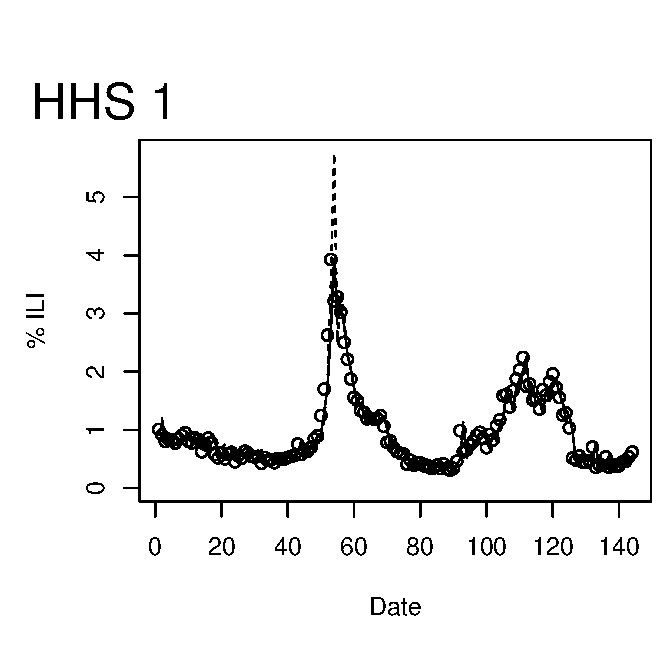
\includegraphics[width=\textwidth]{longitude/figs/nowcastHHS_1.eps}
\end{subfigure}
\begin{subfigure}[b]{0.49\textwidth}
	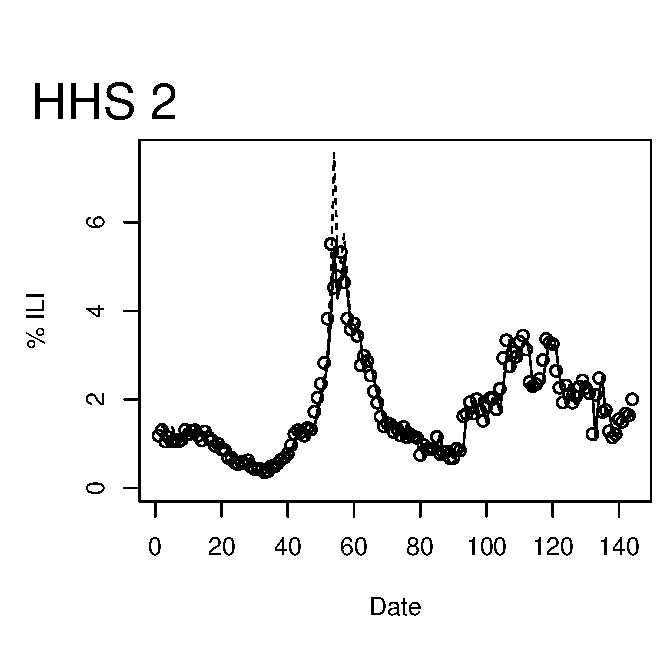
\includegraphics[width=\textwidth]{longitude/figs/nowcastHHS_2.eps}
\end{subfigure}
\\
\begin{subfigure}[b]{0.49\textwidth}
	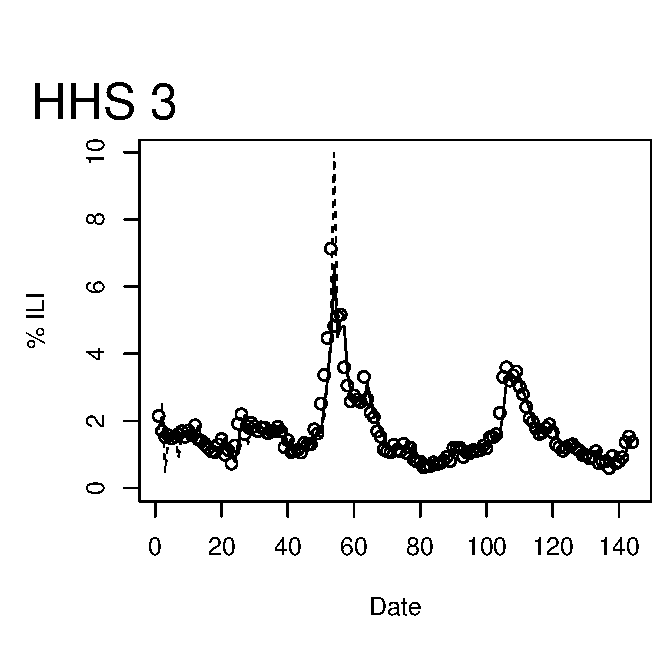
\includegraphics[width=\textwidth]{longitude/figs/nowcastHHS_3.eps}
\end{subfigure}
\begin{subfigure}[b]{0.49\textwidth}
	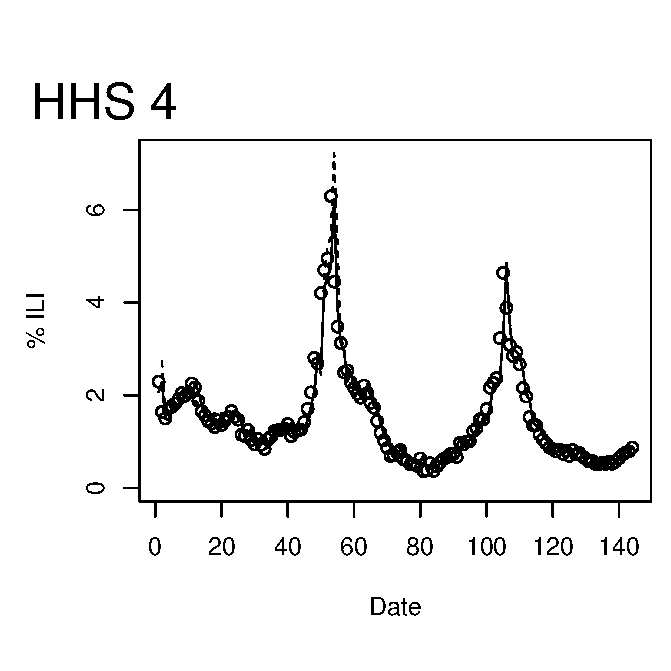
\includegraphics[width=\textwidth]{longitude/figs/nowcastHHS_4.eps}
\end{subfigure}
\\
\begin{subfigure}[b]{0.49\textwidth}
	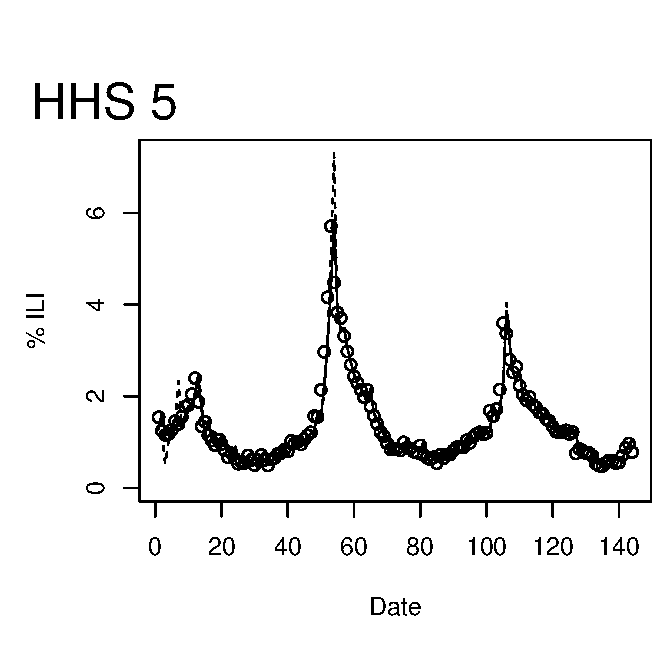
\includegraphics[width=\textwidth]{longitude/figs/nowcastHHS_5.eps}
\end{subfigure}
\begin{subfigure}[b]{0.49\textwidth}
	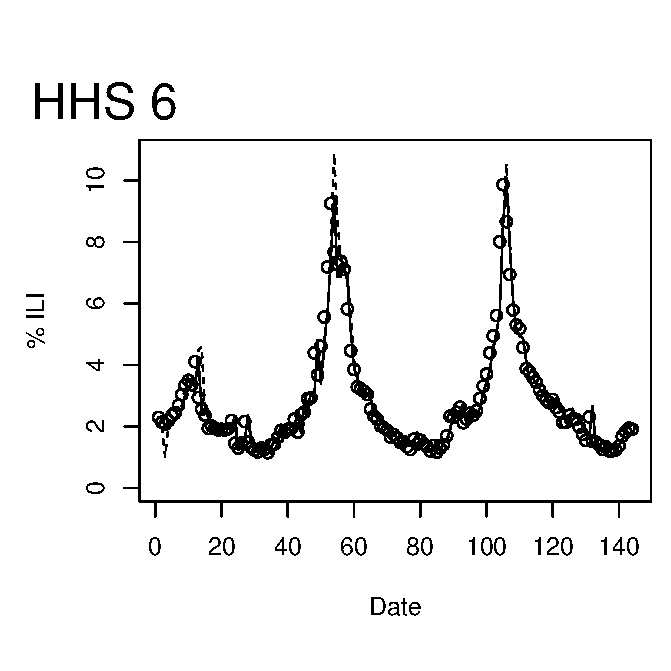
\includegraphics[width=\textwidth]{longitude/figs/nowcastHHS_6.eps}
\end{subfigure}
\end{figure}

\begin{figure}
\centering
\begin{subfigure}[b]{0.49\textwidth}
	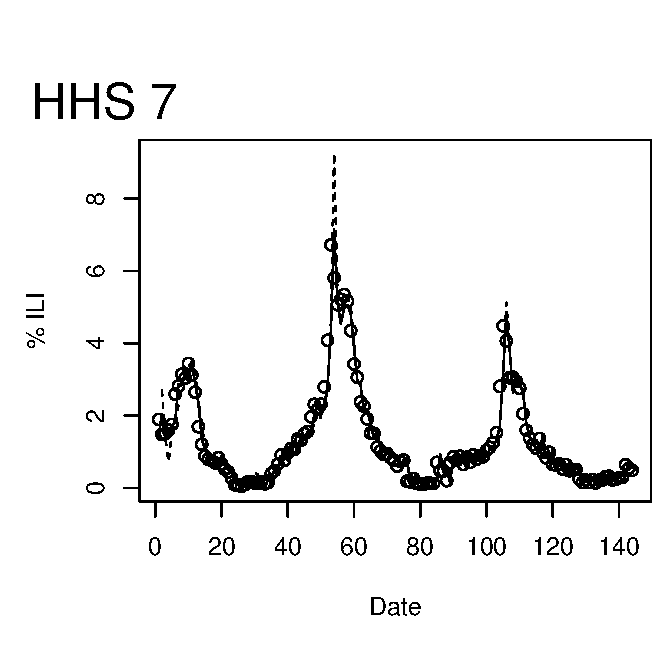
\includegraphics[width=\textwidth]{longitude/figs/nowcastHHS_7.eps}
\end{subfigure}
\begin{subfigure}[b]{0.49\textwidth}
	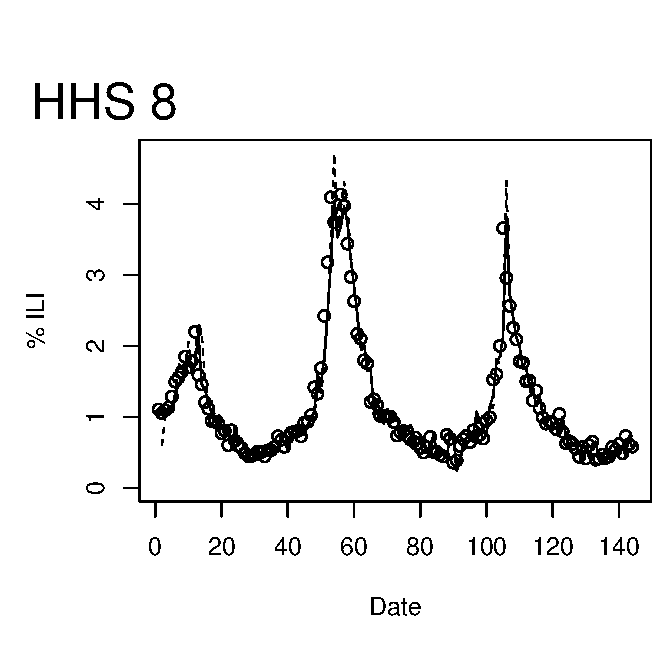
\includegraphics[width=\textwidth]{longitude/figs/nowcastHHS_8.eps}
\end{subfigure}
\\
\begin{subfigure}[b]{0.49\textwidth}
	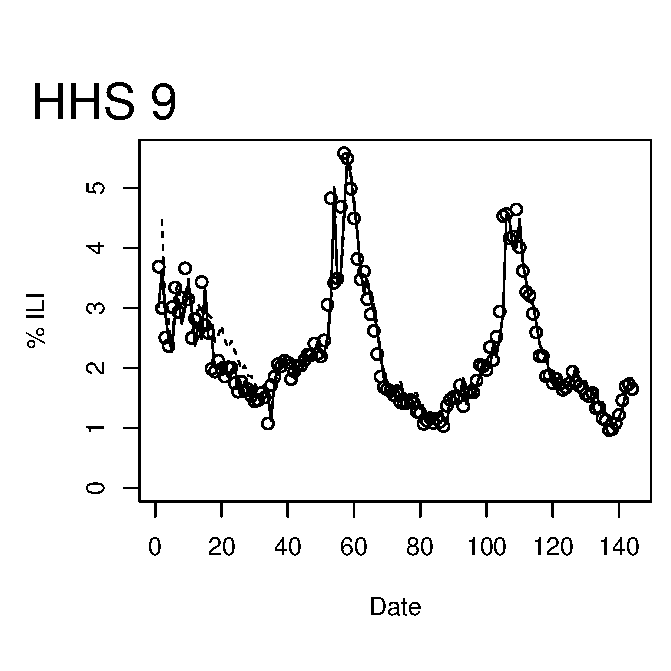
\includegraphics[width=\textwidth]{longitude/figs/nowcastHHS_9.eps}
\end{subfigure}
\begin{subfigure}[b]{0.49\textwidth}
	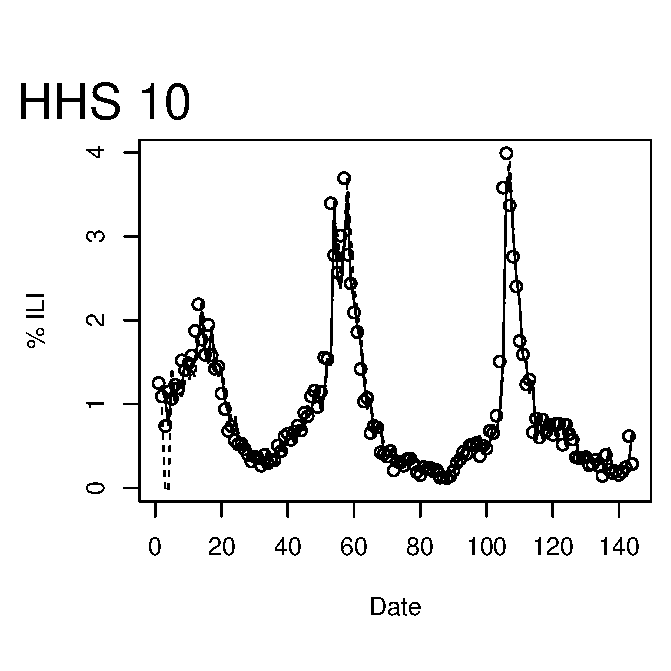
\includegraphics[width=\textwidth]{longitude/figs/nowcastHHS_10.eps}
\end{subfigure}\caption{Comparison of Twitter's forecasting (dashed lines) and retroactive measurements (solid lines) to the CDC's reported Influenza rates (circles) for each of the 10 HHS regions.}
\label{fig:hhs_curves_all}
\end{figure}


\begin{figure}
\centering
\begin{subfigure}[b]{0.49\textwidth}
	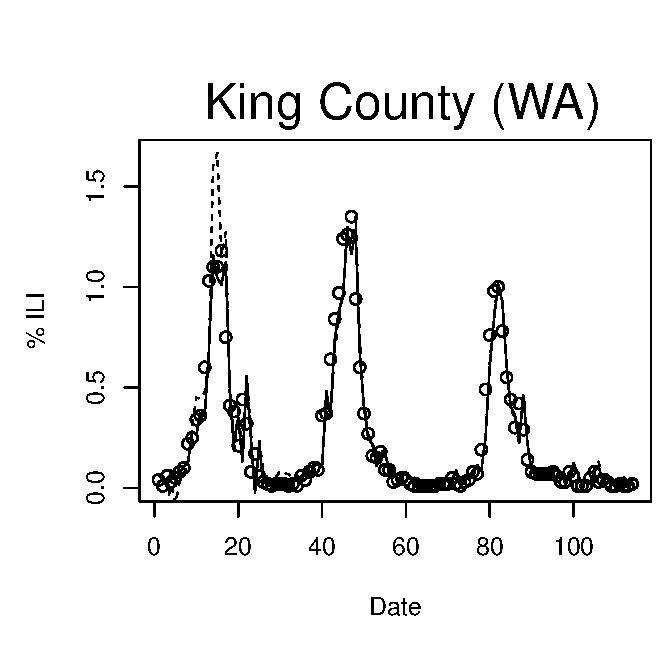
\includegraphics[width=\textwidth]{longitude/figs/nowcastLocal_seattle.eps}
\end{subfigure}
\begin{subfigure}[b]{0.49\textwidth}
	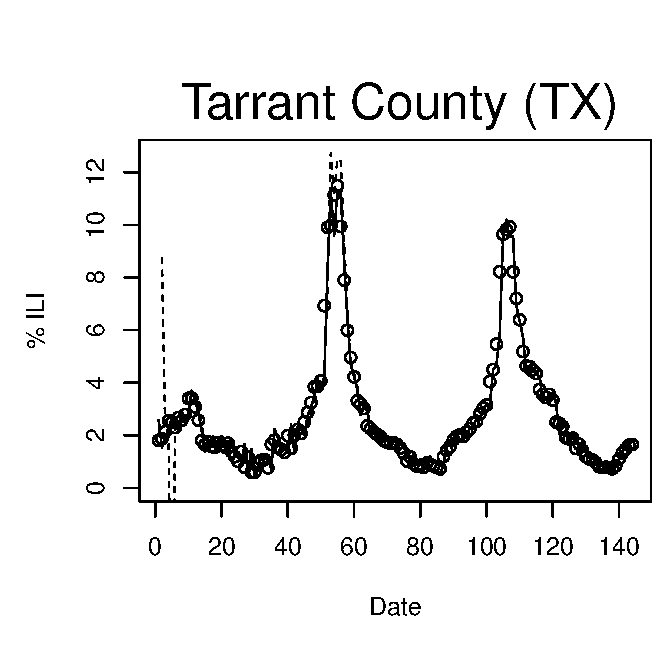
\includegraphics[width=\textwidth]{longitude/figs/nowcastLocal_texas.eps}
\end{subfigure}
\caption{Comparison of Twitter's forecasting (dashed lines) and retroactive measurements (solid lines) to the CDC's reported Influenza rates (circles) for King County and Tarrant County.}
\label{fig:local_curves_all}
\end{figure}
\chapter{A Comparison of Three Types of Message Propagation Models}
\label{appendix:comparetypes}
Here we repeat the analysis in chapter \ref{retweets} on the H7N9 dataset using three different types of propagation models: Retweets (Retweets), Retweets+Hidden flow (Combined), Retweets+Hidden Flow - Spam (No Spam). There are 158364, 139959, and 140174 independent, original messages detected in the models, respectively. 


Due to the large data sizes, we decide to \emph{not} present the statistical significance between the different models as it may be deceptive to the reader. For example, we use the No Spam model in the main paper, which can be predicted using follower count with a correlation of 0.4169. Given the size of the data, the Retweet dataset is different in a statistically significant sense if the correlation is outsize of the range \(.4109 \leq r \leq .4229\) (Fisher z-transformation, two-tailed z-test), approximately a 1.4\% change, which is unlikely to be operationally different.

Here, we repeat the steps described in chapter \ref{retweets} by replicating the modeling of followers, user type and emotions on retweet rates (see table \ref{tab:modelcor3}) and perform keyword model selection (see table \ref{tab:keywordregressionsupplemental}). Instead of doing analysis on an 85\%, 10\%, 5\% split as described in section \ref{tab:combinedfeatures}, we simply work with the full datasets. Thus we do not include the aggregated models, as it would be deceptive to present the fits without a hold out dataset. Note that in 3 out of 4 models, the Combined dataset (the one without spam Tweet copies removed) is the most poorly fit. This loss of preventiveness may be due to a random selection of what Tweets to repost by a simple spam bot compared to the other two datasets, where a human provides some selective pressure in what he or she chooses to retweet.


\begin{table}[]
\centering
\begin{tabular}{|l|r|r|r|r|}
\hline
\multicolumn{1}{|c|}{Model}           & \multicolumn{1}{c|}{Min-N} & \multicolumn{1}{c|}{Retweets} & \multicolumn{1}{c|}{Combined} & \multicolumn{1}{c|}{No Spam} \\ \hline
\multirow{2}{*}{SVMR}                 & 100                        & 0.0132                        & 0.0059                        & -0.0029                      \\ \cline{2-5} 
                                      & 1000                       & -0.0007                       & 0.0013                        & -0.0217                      \\ \hline
\multirow{2}{*}{Regression Tree (2)}  & 100                        & 0.0688                        & 0.0497                        & 0.0747                       \\ \cline{2-5} 
                                      & 1000                       & 0.0653                        & 0.0475                        & 0.0637                       \\ \hline
\multirow{2}{*}{Regression Tree (5)}  & 100                        & 0.0829                        & 0.0719                        & 0.0962                       \\ \cline{2-5} 
                                      & 1000                       & 0.1033                        & 0.0742                        & 0.0927                       \\ \hline
\multirow{2}{*}{Regression Tree (10)} & 100                        & 0.0707                        & 0.0742                        & 0.0642                       \\ \cline{2-5} 
                                      & 1000                       & 0.0891                        & 0.0960                        & 0.1066                       \\ \hline
\multirow{2}{*}{Gradient Boosting}    & 100                        & 0.1552                        & 0.1473                        & 0.1719                       \\ \cline{2-5} 
                                      & 1000                       & 0.1605                        & 0.1408                        & 0.1600                       \\ \hline
\end{tabular}
\caption{Correlation of the output of various regression models used to predict log(retweet) rates given the Tweet's textual content on the three types of tweet propagation: Base API reposts (Retweets), Base reposts plus similar messages (Combined) and Combined with spam removed (No Spam).}
\label{tab:keywordregressionsupplemental}
\end{table}

\begin{table}
\centering
\begin{tabular}{l|r|r|r}
Model & Retweets & Combined & No Spam \\ \hline
Followers & 0.3963  & 0.4151 & 0.4255\\
User Type & 0.2466 & 0.2420 & 0.2503\\
Keyword & 0.1605 & 0.1473 & 0.1719 \\
Emotion & 0.02339 & 0.02119 & 0.02279 \\ \hline
\end{tabular}
\caption{The correlation coefficient of models to predict the propagation count from messages in the H7N9 dataset. }
\label{tab:modelcor3}
\end{table}

%\begin{table}
%\begin{tabular}{l|r|r|r}
%Model & Retweets & Combined & No Spam \\ \hline
%Followers & & & \\
%User Type & & & \\
%Keyword & 0.4191 & 0.4928 & 0.4892 \\
%Emotion & 0.4257 & & \\ \hline
%\end{tabular}
%\label{tab:modelerror3}
%\caption{The mean absolute error of models to predict the propagation count from messages in the H7N9 dataset.}
%\end{table}

\end{appendices}
%\Appendix{Title of the Fifth Appendix}

\section{Introduction}
When in the Course of human events, it becomes necessary for one people  to dissolve the political bands which have connected them with another,  and to assume among the powers of the earth, the separate and equal station  to which the Laws of Nature and of Nature's God entitle them, a decent respect to the opinions of mankind requires that they should declare  the causes which impel them to the separation.

\pagebreak
Some text.
{\lstset{language=Fortran}
\footnotesize
\begin{lstlisting}
      program chaos
c When a LS Fortran program has been compiled and linked into Mac
c application, all information written to the screen WRITE(6,...) or
c WRITE(*,...) appears in a standard Mac window, complete with basic
c menus.
      external fex, jac
      double precision atol, rtol, rwork, t, tout, h
      double precision ttotal, dtout
      dimension h(3), atol(3), rwork(70), iwork(23)
	  character*8 tstart, tend
      neq = 3
	  
	  call time(tstart)
	  write(6,*) "begin integration at  ", tstart
      write(6,*)
	  
c --- Read in the total initial angular momentum.  The total angular
c     momentum H is always unity due to normalization.
	  open(unit = 2, file = 'chaos.data', status = 'unknown')
      read(2,*) h(1), h(2), h(3)
	  
c --- The integration begins at t = 0 and the values are printed at
c     every tout.  tout is incremented below.  ttotal is the length
c     of the entire integration.  The number of recorded values of
c     the integration is given by npoints.
      t = 0.0d0
      tout = 0.0d0
      write(6,*) 'Duration of integration interval, i.e., tfinal?'
      read(6,*) ttotal
      write(6,*)
      write(6,*) 'Number of points for trajectory plot?'
      read(6,*) npoints
      write(6,*)
      dtout = ttotal/dfloat(npoints)
      tout = tout + dtout
	  
c --- Tolerance parameters used by lsoda.
      itol = 2
      rtol = 1.0d-9
      atol(1) = 1.0d-9
      atol(2) = 1.0d-9
      atol(3) = 1.0d-9
	  
c --- Other parameters used by lsoda.  See below.
      itask = 1
      istate = 1
      iopt = 1
      lrw = 70
      liw = 23
      jt = 1

      do 11 kount = 5,10
         rwork(kount) = 0.0d0
         iwork(kount) = 0
  11  continue
      iwork(6) = 100000
	  
	  open(unit = 3, file = 'traj.dat', disp = 'keep',
     &     status = 'unknown')
	 
c --- The actual integration begins here.  Loop on the value of iout.
      do 40 iout = 1, npoints
	  
         call lsoda(fex,neq,h,t,tout,itol,rtol,atol,itask,istate,
     &              iopt,rwork,lrw,iwork,liw,jdum,jt)
	  
c ------ Write the output to the file traj.dat.
         write(3,20) t, h(1), h(2), h(3)
  20     format(f9.1, 3e15.6)

         if (mod(tout,5000.0d0) .eq. 0.0d0) then
            write(6,*) tout
         end if
  
c ------ Check to see that things are going OK.
         if (istate .lt. 0) go to 80
		 
c ------ Set the time at which the integration is next recorded and
c        continue the do-loop.
  40     tout = tout + dtout
  
      write(6,*) 'number of steps taken: ', iwork(11)
      write(6,*) 'number of f evaluations: ', iwork(12)
      write(6,*) 'number of Jacobian evaluations: ', iwork(13)
      write(6,*) 'method order last used: ', iwork(14)
      write(6,*) 'method last used (2 = stiff): ', iwork(19)
      write(6,*) 'value of t at last method switch: ', rwork(15)
      write(6,*)
	 
	  call time(tend)
	  write(6,*) "end integration at  ", tend
      stop
	  
c --- If there is an error, given by istate < 0, write the following.
  80  write(6,90) istate
  90  format(///22h error halt.. istate =,i3)
  
      stop
      end

\end{lstlisting}
}

%%%%%%%%%%%%%%%%%%%%%%%%%%%%%%%%%%%%%%%%%%%%%%%%%%%%%%%%%%%%%%%
% ESM students need to include a Nontechnical Abstract as the %
% last appendix.                                              %
%%%%%%%%%%%%%%%%%%%%%%%%%%%%%%%%%%%%%%%%%%%%%%%%%%%%%%%%%%%%%%%
% This \include command should point to the file containing
% that abstract.
%\include{nontechnical-abstract}
%%%%%%%%%%%%%%%%%%%%%%%%%%%%%%%%%%%%%%%%%%%
} % End of the \allowdisplaybreak command %
%%%%%%%%%%%%%%%%%%%%%%%%%%%%%%%%%%%%%%%%%%%

%%%%%%%%%%%%%%%%
% BIBLIOGRAPHY %
%%%%%%%%%%%%%%%%
% You can use BibTeX or other bibliography facility for your
% bibliography. LaTeX's standard stuff is shown below. If you
% bibtex, then this section should look something like:
	\begin{singlespace}
	\bibliographystyle{GLG-bibstyle}
	\addcontentsline{toc}{chapter}{Bibliography}
	\bibliography{bodnarLibraryFull}
	\end{singlespace}

%\begin{singlespace}
%\begin{thebibliography}{99}
%\addcontentsline{toc}{chapter}{Bibliography}
%\frenchspacing

%\bibitem{Wisdom87} J. Wisdom, ``Rotational Dynamics of Irregularly Shaped Natural Satellites,'' \emph{The Astronomical Journal}, Vol.~94, No.~5, 1987  pp. 1350--1360.

%\bibitem{G&H83} J. Guckenheimer and P. Holmes, \emph{Nonlinear Oscillations, Dynamical Systems, and Bifurcations of Vector Fields}, Springer-Verlag, New York, 1983.

%\end{thebibliography}
%\end{singlespace}

\backmatter

% Vita
\vita{SupplementaryMaterial/Vita}

\end{document}

